\section{Analyse par acte (Chirurgie)} 

\subsection{Acte HZHE0020, Biopsie}

On va ici étudier l'acte HZHE0020 : \textit{Biopsie et/ou brossage cytologique de la paroi du tube digestif ou de conduit biliopancréatique, au cours d'une endoscopie diagnostique}, il s'agit d'un acte chirurgical. La régression \ref{eqn:equation_base} utilisée pour calculer les moyennes conditionnelles du tableau \ref{ambu_HZHE0020} donne un \textbf{R\up{2} ajusté de 0.62}. Par ailleurs, l'estimation des coefficients de ce modèle linéaire est résumée dans le tableau \ref{reg_HZHE0020}.\\

En comparaison, pour l'acte le plus effectué (BFGA0040 : \textit{Extraction extracapsulaire du cristallin par phakoémulsification, avec implantation de cristallin artificiel dans la chambre postérieure de l'oeil}) avec un taux d'ambulatoire de 93.31\%, on trouve un R\up{2} ajusté de 0.11 pour la même regression. Ainsi comme proposé dans la section \ref{intervalle}, l'étude des actes avec un part d'ambulatoire globale ni trop élévée ni trop faible permet de mieux capter les différences entre les catégories d'établissements et au travers des années.\\

\begin{table}[!ht]
\centering
\caption{Pourcentage moyen d'actes HZHE0020 effectués en ambulatoire (\%)} 
\label{ambu_HZHE0020}
\begin{tabular}{r|cccc|c}
  \hline
 & CHU & Privé lucratif & Privé non lucratif & Public & Total \\ 
  \hline
2015 & 40.23 & 86.60 & 75.38 & 51.30 & 73.23 \\ 
  2016 & 43.34 & 86.98 & 76.49 & 53.62 & 74.29 \\ 
  2017 & 45.37 & 86.81 & 75.87 & 54.38 & 72.45 \\ 
  2018 & 47.26 & 86.34 & 75.06 & 56.58 & 70.44 \\ 
  2019 & 48.82 & 87.14 & 76.48 & 57.18 & 69.48 \\ 
  \hline
  Total & 44.81 & 86.77 & 75.86 & 54.58 & 72.34 \\ 
   \hline
\end{tabular}
\bigskip

\begin{tabular}{ccccc}
  \hline
Min. & 1er Qu. & Médiane & 3e Qu. & Max. \\ 
  \hline
0.00 & 56.77 & 79.95 & 89.44 & 100.00000  \\ 
   \hline
\end{tabular}
\end{table}

\begin{table}[!ht]
\centering
\caption{Durée moyenne des séjours} 
\label{dms_HZHE0020}
\begin{tabular}{r|cccc|c}
  \hline
 & CHU & Privé lucratif & Privé non lucratif & Public & Total \\ 
  \hline
2015 & 6.29 & 0.46 & 1.46 & 4.43 & 2.00 \\ 
  2016 & 5.88 & 0.43 & 1.30 & 4.08 & 1.86 \\ 
  2017 & 5.74 & 0.42 & 1.38 & 3.89 & 2.04 \\ 
  2018 & 5.33 & 0.43 & 1.46 & 3.62 & 2.21 \\ 
  2019 & 5.30 & 0.42 & 1.41 & 3.50 & 2.35 \\ 
  \hline
  Total & 5.73 & 0.44 & 1.39 & 3.91 & 2.06 \\ 
   \hline
\end{tabular}

\bigskip

\begin{tabular}{ccccc}
  \hline
Min. & 1er Qu. & Médiane & 3e Qu. & Max. \\ 
  \hline
0.00 & 0.28 & 0.77 & 3.40 & 63.50 \\ 
   \hline
\end{tabular}
\end{table}



Au delà de la forte différence entre le public et le privé dans le pourcentage moyen d'actes effectués en chirurgie ambulatoire de la table \ref{ambu_HZHE0020}, on constate avec le tableau \ref{dms_HZHE0020} que les durées de séjour sont bien plus élevées pour les établissements publics. Ainsi si l'acte n'est pas effectué en ambulatoire, il a plutôt tendance à être associé à un séjour de plusieurs nuits dans le public mais de 1 ou 2 nuits dans le privé. Cela suggère donc une sélection des cas les plus simples par les établissements privés.\\

\begin{table}[!htbp] \centering 
  \caption{Modèles de base appliqué à la part d’actes HZHE0020 en ambulatoire} 
  \label{reg_HZHE0020} 
\begin{tabular}{@{\extracolsep{5pt}}lD{.}{.}{-3} D{.}{.}{-3} D{.}{.}{-3} } 
\\[-1.8ex]\hline 
\hline \\[-1.8ex] 
 & \multicolumn{3}{c}{\textit{Dependent variable:}} \\ 
\cline{2-4} 
\\[-1.8ex] & \multicolumn{3}{c}{Pourcentage d'ambulatoire} \\ 
 & \multicolumn{1}{c}{default} & \multicolumn{1}{c}{robust} & \multicolumn{1}{c}{robust and clustered} \\ 
\\[-1.8ex] & \multicolumn{1}{c}{(1)} & \multicolumn{1}{c}{(2)} & \multicolumn{1}{c}{(3)}\\ 
\hline \\[-1.8ex] 
 Privé lucratif & 41.953^{***} & 41.953^{***} & 41.953^{***} \\ 
  & (0.720) & (1.196) & (2.367) \\ 
  Privé non lucratif & 31.045^{***} & 31.045^{***} & 31.045^{***} \\ 
  & (1.029) & (1.848) & (3.565) \\ 
  Public & 9.765^{***} & 9.765^{***} & 9.765^{***} \\ 
  & (0.774) & (1.296) & (2.600) \\ 
  Constant & 44.812^{***} & 44.812^{***} & 44.812^{***} \\ 
  & (0.656) & (1.120) & (2.271) \\ 
 \hline \\[-1.8ex] 
Observations & \multicolumn{1}{c}{3,693} & \multicolumn{1}{c}{3,693} & \multicolumn{1}{c}{3,693} \\ 
R$^{2}$ & \multicolumn{1}{c}{0.620} & \multicolumn{1}{c}{0.620} & \multicolumn{1}{c}{0.620} \\ 
Adjusted R$^{2}$ & \multicolumn{1}{c}{0.619} & \multicolumn{1}{c}{0.619} & \multicolumn{1}{c}{0.619} \\ 
Residual Std. Error (df = 3689) & \multicolumn{1}{c}{323.276} & \multicolumn{1}{c}{323.276} & \multicolumn{1}{c}{323.276} \\ 
F Statistic (df = 3; 3689) & \multicolumn{1}{c}{2,002.994$^{***}$} & \multicolumn{1}{c}{2,002.994$^{***}$} & \multicolumn{1}{c}{2,002.994$^{***}$} \\ 
\hline 
\hline \\[-1.8ex] 
\textit{Note:}  & \multicolumn{3}{r}{$^{*}$p$<$0.1; $^{**}$p$<$0.05; $^{***}$p$<$0.01} \\ 
\end{tabular} 
\end{table} 

\begin{table}[!htbp] \centering 
\begin{tabular}{@{\extracolsep{5pt}}lD{.}{.}{-3} D{.}{.}{-3} D{.}{.}{-3} } 
\\[-1.8ex]\hline 
\hline \\[-1.8ex] 
 & \multicolumn{3}{c}{\textit{Dependent variable:}} \\ 
\cline{2-4} 
\\[-1.8ex] & \multicolumn{3}{c}{Pourcentage d'ambulatoire} \\ 
 & \multicolumn{1}{c}{default} & \multicolumn{1}{c}{robust} & \multicolumn{1}{c}{robust and clustered} \\ 
\\[-1.8ex] & \multicolumn{1}{c}{(1)} & \multicolumn{1}{c}{(2)} & \multicolumn{1}{c}{(3)}\\ 
\hline \\[-1.8ex] 
 2016 & 1.058 & 1.058 & 1.058^{*} \\ 
  & (1.002) & (1.503) & (0.607) \\ 
  2017 & -0.778 & -0.778 & -0.778 \\ 
  & (1.049) & (1.477) & (0.684) \\ 
  2018 & -2.790^{**} & -2.790^{*} & -2.790^{***} \\ 
  & (1.115) & (1.503) & (0.912) \\ 
  2019 & -3.756^{***} & -3.756^{**} & -3.756^{***} \\ 
  & (1.170) & (1.504) & (0.914) \\ 
  Constant & 73.231^{***} & 73.231^{***} & 73.231^{***} \\ 
  & (0.703) & (1.056) & (1.057) \\ 
 \hline \\[-1.8ex] 
Observations & \multicolumn{1}{c}{3,693} & \multicolumn{1}{c}{3,693} & \multicolumn{1}{c}{3,693} \\ 
R$^{2}$ & \multicolumn{1}{c}{0.006} & \multicolumn{1}{c}{0.006} & \multicolumn{1}{c}{0.006} \\ 
Adjusted R$^{2}$ & \multicolumn{1}{c}{0.005} & \multicolumn{1}{c}{0.005} & \multicolumn{1}{c}{0.005} \\ 
Residual Std. Error (df = 3688) & \multicolumn{1}{c}{522.581} & \multicolumn{1}{c}{522.581} & \multicolumn{1}{c}{522.581} \\ 
F Statistic (df = 4; 3688) & \multicolumn{1}{c}{5.814$^{***}$} & \multicolumn{1}{c}{5.814$^{***}$} & \multicolumn{1}{c}{5.814$^{***}$} \\ 
\hline 
\hline \\[-1.8ex] 
\textit{Note:}  & \multicolumn{3}{r}{$^{*}$p$<$0.1; $^{**}$p$<$0.05; $^{***}$p$<$0.01} \\ 
\end{tabular} 
\end{table} 


\begin{table}[!htbp] \centering 
\scalebox{0.85}{
\begin{tabular}{@{\extracolsep{5pt}}lD{.}{.}{-3} D{.}{.}{-3} D{.}{.}{-3} } 
\\[-1.8ex]\hline 
\hline \\[-1.8ex] 
 & \multicolumn{3}{c}{\textit{Dependent variable:}} \\ 
\cline{2-4} 
\\[-1.8ex] & \multicolumn{3}{c}{Pourcentage d'ambulatoire} \\ 
 & \multicolumn{1}{c}{default} & \multicolumn{1}{c}{robust} & \multicolumn{1}{c}{robust and clustered} \\ 
\\[-1.8ex] & \multicolumn{1}{c}{(1)} & \multicolumn{1}{c}{(2)} & \multicolumn{1}{c}{(3)}\\ 
\hline \\[-1.8ex] 
 Privé lucratif & 46.366^{***} & 46.366^{***} & 46.366^{***} \\ 
  & (1.515) & (2.531) & (2.532) \\ 
  Privé non lucratif & 35.147^{***} & 35.147^{***} & 35.147^{***} \\ 
  & (2.110) & (4.069) & (4.071) \\ 
  Public & 11.070^{***} & 11.070^{***} & 11.070^{***} \\ 
  & (1.671) & (2.757) & (2.758) \\ 
  2016 & 3.107 & 3.107 & 3.107^{***} \\ 
  & (2.004) & (3.428) & (1.167) \\ 
  2017 & 5.141^{**} & 5.141 & 5.141^{***} \\ 
  & (2.016) & (3.381) & (1.372) \\ 
  2018 & 7.029^{***} & 7.029^{**} & 7.029^{***} \\ 
  & (2.042) & (3.404) & (1.467) \\ 
  2019 & 8.589^{***} & 8.589^{**} & 8.589^{***} \\ 
  & (2.101) & (3.629) & (1.938) \\ 
  Privé lucratif*2016 & -2.725 & -2.725 & -2.725^{*} \\ 
  & (2.157) & (3.627) & (1.410) \\ 
  Privé non lucratif*2016 & -1.995 & -1.995 & -1.995 \\ 
  & (3.002) & (5.955) & (2.968) \\ 
  Public*2016 & -0.792 & -0.792 & -0.792 \\ 
  & (2.380) & (4.003) & (1.437) \\ 
  Privé lucratif*2017 & -4.927^{**} & -4.927 & -4.927^{***} \\ 
  & (2.192) & (3.604) & (1.640) \\ 
  Privé non lucratif*2017 & -4.648 & -4.648 & -4.648 \\ 
  & (3.105) & (5.832) & (3.160) \\ 
  Public*2017 & -2.062 & -2.062 & -2.062 \\ 
  & (2.390) & (3.938) & (1.692) \\ 
  Privé lucratif*2018 & -7.286^{***} & -7.286^{**} & -7.286^{***} \\ 
  & (2.258) & (3.710) & (1.983) \\ 
  Privé non lucratif*2018 & -7.345^{**} & -7.345 & -7.345^{**} \\ 
  & (3.246) & (5.736) & (3.702) \\ 
  Public*2018 & -1.749 & -1.749 & -1.749 \\ 
  & (2.415) & (3.974) & (1.971) \\ 
  Privé lucratif*2019 & -8.046^{***} & -8.046^{**} & -8.046^{***} \\ 
  & (2.357) & (3.893) & (2.310) \\ 
  Privé non lucratif*2019 & -7.491^{**} & -7.491 & -7.491^{**} \\ 
  & (3.359) & (5.532) & (3.740) \\ 
  Public*2019 & -2.708 & -2.708 & -2.708 \\ 
  & (2.466) & (4.156) & (2.363) \\ 
  Constant & 40.232^{***} & 40.232^{***} & 40.232^{***} \\ 
  & (1.408) & (2.354) & (2.355) \\ 
 \hline \\[-1.8ex] 
Observations & \multicolumn{1}{c}{3,693} & \multicolumn{1}{c}{3,693} & \multicolumn{1}{c}{3,693} \\ 
R$^{2}$ & \multicolumn{1}{c}{0.625} & \multicolumn{1}{c}{0.625} & \multicolumn{1}{c}{0.625} \\ 
Adjusted R$^{2}$ & \multicolumn{1}{c}{0.623} & \multicolumn{1}{c}{0.623} & \multicolumn{1}{c}{0.623} \\ 
Residual Std. Error (df = 3673) & \multicolumn{1}{c}{321.823} & \multicolumn{1}{c}{321.823} & \multicolumn{1}{c}{321.823} \\ 
F Statistic (df = 19; 3673) & \multicolumn{1}{c}{321.723$^{***}$} & \multicolumn{1}{c}{321.723$^{***}$} & \multicolumn{1}{c}{321.723$^{***}$} \\ 
\hline 
\hline \\[-1.8ex] 
\end{tabular} 
}
\end{table} 

\clearpage

Au vu des résultats précédent suggèrant une sélection des cas les plus simples par les établissements privés, on va effectuer de nouveau la régression sur la part d'ambulatoire mais en ajoutant un contrôle sur la sévérité des actes. Les estimations sont dans la table \ref{reg_A9_HZHE0020},  la variable de contrôle a l'air pertinente, sa prise en compte permet de diminuer l'écart entre les hôpitaux publics et les hôpitaux privés.\\

\begin{table}[!htbp] \centering 
  \caption{Modèles de base avec contrôle par A9 (acte HZHE0020)} 
  \label{reg_A9_HZHE0020} 
\begin{tabular}{@{\extracolsep{5pt}}lD{.}{.}{-3} D{.}{.}{-3} D{.}{.}{-3} } 
\\[-1.8ex]\hline 
\hline \\[-1.8ex] 
 & \multicolumn{3}{c}{\textit{Dependent variable:}} \\ 
\cline{2-4} 
\\[-1.8ex] & \multicolumn{3}{c}{Pourcentage d'ambulatoire} \\ 
 & \multicolumn{1}{c}{default} & \multicolumn{1}{c}{robust} & \multicolumn{1}{c}{robust and clustered} \\ 
\\[-1.8ex] & \multicolumn{1}{c}{(1)} & \multicolumn{1}{c}{(2)} & \multicolumn{1}{c}{(3)}\\ 
\hline \\[-1.8ex] 
 Privé lucratif & 36.565^{***} & 36.565^{***} & 36.565^{***} \\ 
  & (0.948) & (1.589) & (3.120) \\ 
  Privé non lucratif & 29.359^{***} & 29.359^{***} & 29.359^{***} \\ 
  & (1.037) & (1.784) & (3.437) \\ 
  Public & 11.319^{***} & 11.319^{***} & 11.319^{***} \\ 
  & (0.787) & (1.336) & (2.658) \\ 
  A9 & -0.654^{***} & -0.654^{***} & -0.654^{***} \\ 
  & (0.076) & (0.122) & (0.237) \\ 
  Constant & 52.226^{***} & 52.226^{***} & 52.226^{***} \\ 
  & (1.077) & (1.790) & (3.532) \\ 
 \hline \\[-1.8ex] 
Observations & \multicolumn{1}{c}{3,693} & \multicolumn{1}{c}{3,693} & \multicolumn{1}{c}{3,693} \\ 
R$^{2}$ & \multicolumn{1}{c}{0.627} & \multicolumn{1}{c}{0.627} & \multicolumn{1}{c}{0.627} \\ 
Adjusted R$^{2}$ & \multicolumn{1}{c}{0.627} & \multicolumn{1}{c}{0.627} & \multicolumn{1}{c}{0.627} \\ 
Residual Std. Error (df = 3688) & \multicolumn{1}{c}{320.105} & \multicolumn{1}{c}{320.105} & \multicolumn{1}{c}{320.105} \\ 
F Statistic (df = 4; 3688) & \multicolumn{1}{c}{1,550.765$^{***}$} & \multicolumn{1}{c}{1,550.765$^{***}$} & \multicolumn{1}{c}{1,550.765$^{***}$} \\ 
\hline 
\hline \\[-1.8ex] 
\textit{Note:}  & \multicolumn{3}{r}{$^{*}$p$<$0.1; $^{**}$p$<$0.05; $^{***}$p$<$0.01} \\ 
\end{tabular} 
\end{table}

\begin{table}[!htbp] \centering 
\begin{tabular}{@{\extracolsep{5pt}}lD{.}{.}{-3} D{.}{.}{-3} D{.}{.}{-3} } 
\\[-1.8ex]\hline 
\hline \\[-1.8ex] 
 & \multicolumn{3}{c}{\textit{Dependent variable:}} \\ 
\cline{2-4} 
\\[-1.8ex] & \multicolumn{3}{c}{Pourcentage d'ambulatoire} \\ 
 & \multicolumn{1}{c}{default} & \multicolumn{1}{c}{robust} & \multicolumn{1}{c}{robust and clustered} \\ 
\\[-1.8ex] & \multicolumn{1}{c}{(1)} & \multicolumn{1}{c}{(2)} & \multicolumn{1}{c}{(3)}\\ 
\hline \\[-1.8ex] 
 2016 & 1.689^{**} & 1.689 & 1.689^{***} \\ 
  & (0.731) & (1.266) & (0.563) \\ 
  2017 & 2.105^{***} & 2.105^{*} & 2.105^{***} \\ 
  & (0.768) & (1.245) & (0.632) \\ 
  2018 & 2.883^{***} & 2.883^{**} & 2.883^{***} \\ 
  & (0.820) & (1.299) & (0.867) \\ 
  2019 & 3.849^{***} & 3.849^{***} & 3.849^{***} \\ 
  & (0.865) & (1.290) & (0.866) \\ 
  A9 & -2.670^{***} & -2.670^{***} & -2.670^{***} \\ 
  & (0.047) & (0.073) & (0.143) \\ 
  Constant & 90.225^{***} & 90.225^{***} & 90.225^{***} \\ 
  & (0.594) & (1.004) & (1.219) \\ 
 \hline \\[-1.8ex] 
Observations & \multicolumn{1}{c}{3,693} & \multicolumn{1}{c}{3,693} & \multicolumn{1}{c}{3,693} \\ 
R$^{2}$ & \multicolumn{1}{c}{0.471} & \multicolumn{1}{c}{0.471} & \multicolumn{1}{c}{0.471} \\ 
Adjusted R$^{2}$ & \multicolumn{1}{c}{0.470} & \multicolumn{1}{c}{0.470} & \multicolumn{1}{c}{0.470} \\ 
Residual Std. Error (df = 3687) & \multicolumn{1}{c}{381.408} & \multicolumn{1}{c}{381.408} & \multicolumn{1}{c}{381.408} \\ 
F Statistic (df = 5; 3687) & \multicolumn{1}{c}{656.010$^{***}$} & \multicolumn{1}{c}{656.010$^{***}$} & \multicolumn{1}{c}{656.010$^{***}$} \\ 
\hline 
\hline \\[-1.8ex] 
\textit{Note:}  & \multicolumn{3}{r}{$^{*}$p$<$0.1; $^{**}$p$<$0.05; $^{***}$p$<$0.01} \\ 
\end{tabular} 
\end{table}

\begin{table}[!htbp] \centering 
\scalebox{0.82}{
\begin{tabular}{@{\extracolsep{5pt}}lD{.}{.}{-3} D{.}{.}{-3} D{.}{.}{-3} } 
\\[-1.8ex]\hline 
\hline \\[-1.8ex] 
 & \multicolumn{3}{c}{\textit{Dependent variable:}} \\ 
\cline{2-4} 
\\[-1.8ex] & \multicolumn{3}{c}{Pourcentage d'ambulatoire} \\ 
 & \multicolumn{1}{c}{default} & \multicolumn{1}{c}{robust} & \multicolumn{1}{c}{robust and clustered} \\ 
\\[-1.8ex] & \multicolumn{1}{c}{(1)} & \multicolumn{1}{c}{(2)} & \multicolumn{1}{c}{(3)}\\ 
\hline \\[-1.8ex] 
 Privé lucratif & 40.566^{***} & 40.566^{***} & 40.566^{***} \\ 
  & (1.616) & (2.731) & (3.188) \\ 
  Privé non lucratif & 32.775^{***} & 32.775^{***} & 32.775^{***} \\ 
  & (2.100) & (3.982) & (3.994) \\ 
  Public & 12.463^{***} & 12.463^{***} & 12.463^{***} \\ 
  & (1.658) & (2.791) & (2.810) \\ 
  2016 & 3.224 & 3.224 & 3.224^{***} \\ 
  & (1.980) & (3.460) & (1.176) \\ 
  2017 & 5.406^{***} & 5.406 & 5.406^{***} \\ 
  & (1.992) & (3.406) & (1.376) \\ 
  2018 & 7.543^{***} & 7.543^{**} & 7.543^{***} \\ 
  & (2.018) & (3.419) & (1.472) \\ 
  2019 & 9.075^{***} & 9.075^{**} & 9.075^{***} \\ 
  & (2.076) & (3.643) & (1.946) \\ 
  A9 & -0.725^{***} & -0.725^{***} & -0.725^{***} \\ 
  & (0.076) & (0.121) & (0.237) \\ 
  Privé lucratif*2016 & -2.722 & -2.722 & -2.722^{*} \\ 
  & (2.131) & (3.640) & (1.407) \\ 
  Privé non lucratif*2016 & -1.923 & -1.923 & -1.923 \\ 
  & (2.966) & (5.788) & (2.904) \\ 
  Public*2016 & -0.663 & -0.663 & -0.663 \\ 
  & (2.351) & (4.033) & (1.444) \\ 
  Privé lucratif*2017 & -5.031^{**} & -5.031 & -5.031^{***} \\ 
  & (2.166) & (3.609) & (1.633) \\ 
  Privé non lucratif*2017 & -4.049 & -4.049 & -4.049 \\ 
  & (3.069) & (5.612) & (3.029) \\ 
  Public*2017 & -1.664 & -1.664 & -1.664 \\ 
  & (2.362) & (3.964) & (1.690) \\ 
  Privé lucratif*2018 & -7.671^{***} & -7.671^{**} & -7.671^{***} \\ 
  & (2.232) & (3.708) & (1.978) \\ 
  Privé non lucratif*2018 & -6.102^{*} & -6.102 & -6.102^{*} \\ 
  & (3.210) & (5.532) & (3.455) \\ 
  Public*2018 & -1.277 & -1.277 & -1.277 \\ 
  & (2.386) & (3.991) & (1.983) \\ 
  Privé lucratif*2019 & -8.412^{***} & -8.412^{**} & -8.412^{***} \\ 
  & (2.329) & (3.889) & (2.306) \\ 
  Privé non lucratif*2019 & -6.086^{*} & -6.086 & -6.086^{*} \\ 
  & (3.322) & (5.322) & (3.510) \\ 
  Public*2019 & -2.085 & -2.085 & -2.085 \\ 
  & (2.438) & (4.169) & (2.380) \\ 
  Constant & 48.180^{***} & 48.180^{***} & 48.180^{***} \\ 
  & (1.623) & (2.721) & (3.515) \\ 
 \hline \\[-1.8ex] 
Observations & \multicolumn{1}{c}{3,693} & \multicolumn{1}{c}{3,693} & \multicolumn{1}{c}{3,693} \\ 
R$^{2}$ & \multicolumn{1}{c}{0.634} & \multicolumn{1}{c}{0.634} & \multicolumn{1}{c}{0.634} \\ 
Adjusted R$^{2}$ & \multicolumn{1}{c}{0.632} & \multicolumn{1}{c}{0.632} & \multicolumn{1}{c}{0.632} \\ 
Residual Std. Error (df = 3672) & \multicolumn{1}{c}{317.977} & \multicolumn{1}{c}{317.977} & \multicolumn{1}{c}{317.977} \\ 
F Statistic (df = 20; 3672) & \multicolumn{1}{c}{317.595$^{***}$} & \multicolumn{1}{c}{317.595$^{***}$} & \multicolumn{1}{c}{317.595$^{***}$} \\ 
\hline 
\hline \\[-1.8ex] 
\end{tabular} 
}
\end{table} 

\clearpage

On ajoute le contrôle par l'enseignement et la recherche (tableaux \ref{reg_controle_A1_H}), malgré ce contrôle, il reste toujours des écarts significatifs entre les catégories d'établissements, en particulier entre le public et le privé.\\


\begin{table}[!htbp] \centering 
  \caption{Modèle de base avec contrôle par A9, A10 et A11 (+interaction entre A10 et A11)} 
  \label{reg_controle_A1_H} 
\begin{tabular}{@{\extracolsep{5pt}}lD{.}{.}{-3} D{.}{.}{-3} D{.}{.}{-3} } 
\\[-1.8ex]\hline 
\hline \\[-1.8ex] 
 & \multicolumn{3}{c}{\textit{Dependent variable:}} \\ 
\cline{2-4} 
\\[-1.8ex] & \multicolumn{3}{c}{Pourcentage d'ambulatoire} \\ 
 & \multicolumn{1}{c}{default} & \multicolumn{1}{c}{robust} & \multicolumn{1}{c}{robust and clustered} \\ 
\\[-1.8ex] & \multicolumn{1}{c}{(1)} & \multicolumn{1}{c}{(2)} & \multicolumn{1}{c}{(3)}\\ 
\hline \\[-1.8ex] 
 Privé lucratif & 32.883^{***} & 32.883^{***} & 32.883^{***} \\ 
  & (1.679) & (2.691) & (5.050) \\ 
  Privé non lucratif & 26.310^{***} & 26.310^{***} & 26.310^{***} \\ 
  & (1.596) & (2.566) & (4.797) \\ 
  Public & 8.597^{***} & 8.597^{***} & 8.597^{*} \\ 
  & (1.536) & (2.472) & (4.711) \\ 
  A9 & -0.684^{***} & -0.684^{***} & -0.684^{***} \\ 
  & (0.076) & (0.124) & (0.239) \\ 
  A10 & -10.698^{***} & -10.698^{***} & -10.698^{***} \\ 
  & (1.657) & (2.121) & (4.130) \\ 
  A11 & 0.014 & 0.014 & 0.014 \\ 
  & (0.618) & (1.339) & (2.536) \\ 
  A10*A11 & 7.098^{***} & 7.098^{***} & 7.098^{**} \\ 
  & (1.512) & (1.611) & (3.056) \\ 
  Constant & 56.000^{***} & 56.000^{***} & 56.000^{***} \\ 
  & (1.761) & (2.815) & (5.292) \\ 
 \hline \\[-1.8ex] 
Observations & \multicolumn{1}{c}{3,693} & \multicolumn{1}{c}{3,693} & \multicolumn{1}{c}{3,693} \\ 
R$^{2}$ & \multicolumn{1}{c}{0.631} & \multicolumn{1}{c}{0.631} & \multicolumn{1}{c}{0.631} \\ 
Adjusted R$^{2}$ & \multicolumn{1}{c}{0.631} & \multicolumn{1}{c}{0.631} & \multicolumn{1}{c}{0.631} \\ 
Residual Std. Error (df = 3685) & \multicolumn{1}{c}{318.411} & \multicolumn{1}{c}{318.411} & \multicolumn{1}{c}{318.411} \\ 
F Statistic (df = 7; 3685) & \multicolumn{1}{c}{901.654$^{***}$} & \multicolumn{1}{c}{901.654$^{***}$} & \multicolumn{1}{c}{901.654$^{***}$} \\ 
\hline 
\hline \\[-1.8ex] 
\textit{Note:}  & \multicolumn{3}{r}{$^{*}$p$<$0.1; $^{**}$p$<$0.05; $^{***}$p$<$0.01} \\ 
\end{tabular} 
\end{table}

\begin{table}[!htbp] \centering  
\begin{tabular}{@{\extracolsep{5pt}}lD{.}{.}{-3} D{.}{.}{-3} D{.}{.}{-3} } 
\\[-1.8ex]\hline 
\hline \\[-1.8ex] 
 & \multicolumn{3}{c}{\textit{Dependent variable:}} \\ 
\cline{2-4} 
\\[-1.8ex] & \multicolumn{3}{c}{Pourcentage d'ambulatoire} \\ 
 & \multicolumn{1}{c}{default} & \multicolumn{1}{c}{robust} & \multicolumn{1}{c}{robust and clustered} \\ 
\\[-1.8ex] & \multicolumn{1}{c}{(1)} & \multicolumn{1}{c}{(2)} & \multicolumn{1}{c}{(3)}\\ 
\hline \\[-1.8ex] 
 2016 & 1.578^{**} & 1.578 & 1.578^{***} \\ 
  & (0.672) & (1.166) & (0.553) \\ 
  2017 & 2.252^{***} & 2.252^{**} & 2.252^{***} \\ 
  & (0.706) & (1.147) & (0.623) \\ 
  2018 & 3.224^{***} & 3.224^{***} & 3.224^{***} \\ 
  & (0.753) & (1.208) & (0.846) \\ 
  2019 & 4.227^{***} & 4.227^{***} & 4.227^{***} \\ 
  & (0.794) & (1.188) & (0.858) \\ 
  A9 & -2.349^{***} & -2.349^{***} & -2.349^{***} \\ 
  & (0.045) & (0.068) & (0.133) \\ 
  A10 & -22.134^{***} & -22.134^{***} & -22.134^{***} \\ 
  & (1.720) & (2.069) & (3.737) \\ 
  A11 & -0.516 & -0.516 & -0.516 \\ 
  & (0.644) & (1.478) & (2.741) \\ 
  A10*A11 & 7.300^{***} & 7.300^{***} & 7.300^{**} \\ 
  & (1.594) & (2.189) & (3.620) \\ 
  Constant & 90.291^{***} & 90.291^{***} & 90.291^{***} \\ 
  & (0.546) & (0.921) & (1.056) \\ 
 \hline \\[-1.8ex] 
Observations & \multicolumn{1}{c}{3,693} & \multicolumn{1}{c}{3,693} & \multicolumn{1}{c}{3,693} \\ 
R$^{2}$ & \multicolumn{1}{c}{0.554} & \multicolumn{1}{c}{0.554} & \multicolumn{1}{c}{0.554} \\ 
Adjusted R$^{2}$ & \multicolumn{1}{c}{0.553} & \multicolumn{1}{c}{0.553} & \multicolumn{1}{c}{0.553} \\ 
Residual Std. Error (df = 3684) & \multicolumn{1}{c}{350.215} & \multicolumn{1}{c}{350.215} & \multicolumn{1}{c}{350.215} \\ 
F Statistic (df = 8; 3684) & \multicolumn{1}{c}{572.421$^{***}$} & \multicolumn{1}{c}{572.421$^{***}$} & \multicolumn{1}{c}{572.421$^{***}$} \\ 
\hline 
\hline \\[-1.8ex] 
\textit{Note:}  & \multicolumn{3}{r}{$^{*}$p$<$0.1; $^{**}$p$<$0.05; $^{***}$p$<$0.01} \\ 
\end{tabular} 
\end{table} 

\begin{table}[!htbp] \centering
\scalebox{0.75}{
\begin{tabular}{@{\extracolsep{5pt}}lD{.}{.}{-3} D{.}{.}{-3} D{.}{.}{-3} } 
\\[-1.8ex]\hline 
\hline \\[-1.8ex] 
 & \multicolumn{3}{c}{\textit{Dependent variable:}} \\ 
\cline{2-4} 
\\[-1.8ex] & \multicolumn{3}{c}{Pourcentage d'ambulatoire} \\ 
 & \multicolumn{1}{c}{default} & \multicolumn{1}{c}{robust} & \multicolumn{1}{c}{robust and clustered} \\ 
\\[-1.8ex] & \multicolumn{1}{c}{(1)} & \multicolumn{1}{c}{(2)} & \multicolumn{1}{c}{(3)}\\ 
\hline \\[-1.8ex] 
 Privé lucratif & 36.138^{***} & 36.138^{***} & 36.138^{***} \\ 
  & (2.113) & (3.489) & (5.062) \\ 
  Privé non lucratif & 29.088^{***} & 29.088^{***} & 29.088^{***} \\ 
  & (2.419) & (4.304) & (5.106) \\ 
  Public & 8.927^{***} & 8.927^{**} & 8.927^{*} \\ 
  & (2.101) & (3.491) & (4.780) \\ 
  2016 & 3.111 & 3.111 & 3.111^{**} \\ 
  & (1.970) & (3.437) & (1.218) \\ 
  2017 & 5.351^{***} & 5.351 & 5.351^{***} \\ 
  & (1.982) & (3.423) & (1.366) \\ 
  2018 & 7.624^{***} & 7.624^{**} & 7.624^{***} \\ 
  & (2.009) & (3.440) & (1.474) \\ 
  2019 & 9.273^{***} & 9.273^{**} & 9.273^{***} \\ 
  & (2.068) & (3.637) & (1.979) \\ 
  A9 & -0.757^{***} & -0.757^{***} & -0.757^{***} \\ 
  & (0.076) & (0.123) & (0.239) \\ 
  A10 & -11.008^{***} & -11.008^{***} & -11.008^{***} \\ 
  & (1.646) & (2.116) & (4.148) \\ 
  A11 & -0.032 & -0.032 & -0.032 \\ 
  & (0.623) & (1.299) & (2.480) \\ 
  Privé lucratif*2016 & -2.603 & -2.603 & -2.603^{*} \\ 
  & (2.120) & (3.618) & (1.443) \\ 
  Privé non lucratif*2016 & -1.927 & -1.927 & -1.927 \\ 
  & (2.963) & (5.670) & (2.926) \\ 
  Public*2016 & -0.420 & -0.420 & -0.420 \\ 
  & (2.339) & (4.012) & (1.480) \\ 
  Privé lucratif*2017 & -4.966^{**} & -4.966 & -4.966^{***} \\ 
  & (2.155) & (3.626) & (1.630) \\ 
  Privé non lucratif*2017 & -3.983 & -3.983 & -3.983 \\ 
  & (3.051) & (5.516) & (3.038) \\ 
  Public*2017 & -1.441 & -1.441 & -1.441 \\ 
  & (2.349) & (3.976) & (1.683) \\ 
  Privé lucratif*2018 & -7.745^{***} & -7.745^{**} & -7.745^{***} \\ 
  & (2.221) & (3.728) & (1.981) \\ 
  Privé non lucratif*2018 & -6.075^{*} & -6.075 & -6.075^{*} \\ 
  & (3.192) & (5.431) & (3.477) \\ 
  Public*2018 & -1.187 & -1.187 & -1.187 \\ 
  & (2.375) & (4.007) & (1.981) \\ 
  Privé lucratif*2019 & -8.605^{***} & -8.605^{**} & -8.605^{***} \\ 
  & (2.319) & (3.884) & (2.335) \\ 
  Privé non lucratif*2019 & -6.191^{*} & -6.191 & -6.191^{*} \\ 
  & (3.303) & (5.318) & (3.598) \\ 
  Public*2019 & -2.096 & -2.096 & -2.096 \\ 
  & (2.426) & (4.161) & (2.399) \\ 
  A10*A11 & 6.881^{***} & 6.881^{***} & 6.881^{**} \\ 
  & (1.506) & (1.592) & (3.055) \\ 
  Constant & 52.705^{***} & 52.705^{***} & 52.705^{***} \\ 
  & (2.123) & (3.479) & (5.251) \\ 
 \hline \\[-1.8ex] 
Observations & \multicolumn{1}{c}{3,693} & \multicolumn{1}{c}{3,693} & \multicolumn{1}{c}{3,693} \\ 
R$^{2}$ & \multicolumn{1}{c}{0.638} & \multicolumn{1}{c}{0.638} & \multicolumn{1}{c}{0.638} \\ 
Adjusted R$^{2}$ & \multicolumn{1}{c}{0.636} & \multicolumn{1}{c}{0.636} & \multicolumn{1}{c}{0.636} \\ 
Residual Std. Error (df = 3669) & \multicolumn{1}{c}{316.140} & \multicolumn{1}{c}{316.140} & \multicolumn{1}{c}{316.140} \\ 
F Statistic (df = 23; 3669) & \multicolumn{1}{c}{281.379$^{***}$} & \multicolumn{1}{c}{281.379$^{***}$} & \multicolumn{1}{c}{281.379$^{***}$} \\ 
\hline 
\hline \\[-1.8ex] 
\end{tabular} 
}
\end{table} 

\clearpage

Du fait que la tarification est agrégée au niveau d'un acte CCAM, on ne peut pas l'utiliser dans l'étude d'un acte unique. Pour le modèle de contrôle par interaction avec \textit{A9}, on va donc utiliser le modèle \ref{eqn:controle_inter2}. lLes estimations des coefficients sont consultables dans la table \ref{controle_inter_HZHE0020} et les courbes de la part d'actes en ambulatoire selon \textit{A9} pour chaque catégorie d'établissement sont dans la figure \ref{courbe_inter_HZHE0020}. On observe que les établissements privés dépendent plus fortement de \textit{A9}, traduisant la sévérité des actes. La droite correspondant aux CHU a un  coefficient positif cela est probablement du au fait que l'effectif de cette catégorie est plus faible, ainsi l'estimation s'effectue sur peu de données regroupées autour d'une valeur de \textit{A9} assez élevée.\\

\begin{equation} \label{eqn:controle_inter2}
    \left\{
    \begin{array}{ll}
        Y^{inter_2}_i = Y^{inter}_i + \beta_{A10}.A10_i + \beta_{A11}.A11_i + \beta_{A10*A11}.A10_i.A11_i\\
        Y^{inter}_i \text{  donné par l'équation \ref{eqn:int}}
    \end{array}
\right.
\end{equation}

\begin{figure}[!ht]
    \centering
    \caption{Estimation de la part d'ambulatoire en fonction de A9}
    \label{courbe_inter_HZHE0020}
    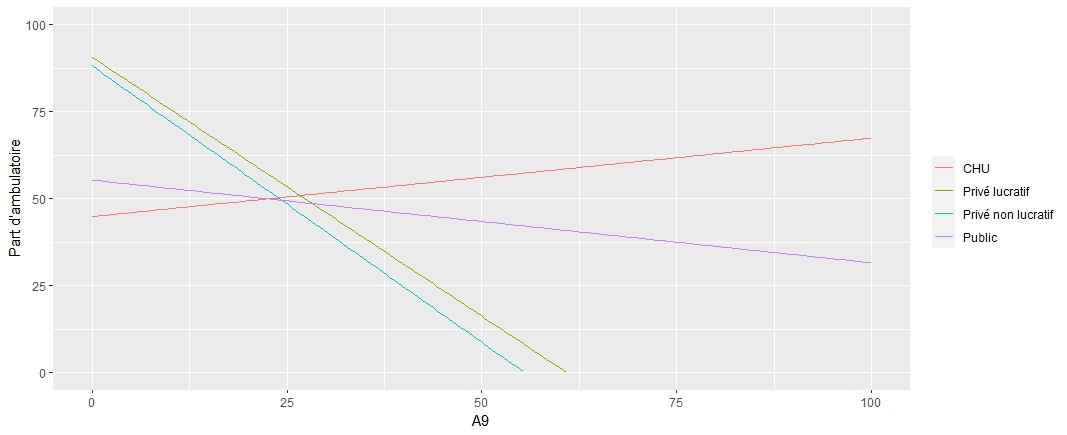
\includegraphics[scale=0.7]{Images/A9_inter_1.jpeg}
\end{figure}

Points d'intersection (A9, Part d'ambulatoire):

\begin{itemize}
    \item CHU - Privé lucratif : $(26.73273,50.89212)$
    \item CHU - Privé non lucratif : $(23.87571,50.24782)$
    \item CHU - Public : $(22.60185,49.96055)$
    \item Privé lucratif - Public : $(28.26316,48.6146 )$
    \item Privé non lucratif - Public : $(24.31254,49.55384 )$
\end{itemize}

\begin{table}[!htbp] \centering 
  \caption{Modèle \ref{eqn:controle_inter2} avec contrôle par interaction de A9} 
  \label{controle_inter_HZHE0020} 
\begin{tabular}{@{\extracolsep{5pt}}lD{.}{.}{-3} D{.}{.}{-3} D{.}{.}{-3} } 
\\[-1.8ex]\hline 
\hline \\[-1.8ex] 
 & \multicolumn{3}{c}{\textit{Dependent variable:}} \\ 
\cline{2-4} 
\\[-1.8ex] & \multicolumn{3}{c}{Pourcentage d'ambulatoire} \\ 
 & \multicolumn{1}{c}{default} & \multicolumn{1}{c}{robust} & \multicolumn{1}{c}{robust and clustered} \\ 
\\[-1.8ex] & \multicolumn{1}{c}{(1)} & \multicolumn{1}{c}{(2)} & \multicolumn{1}{c}{(3)}\\ 
\hline \\[-1.8ex] 
 Privé lucratif & 45.811^{***} & 45.811^{***} & 45.811^{**} \\ 
  & (7.127) & (11.927) & (18.804) \\ 
  Privé non lucratif & 43.315^{***} & 43.315^{***} & 43.315^{**} \\ 
  & (7.294) & (12.106) & (19.198) \\ 
  Public & 10.471 & 10.471 & 10.471 \\ 
  & (7.244) & (12.081) & (19.238) \\ 
  A9 & 0.226 & 0.226 & 0.226 \\ 
  & (0.600) & (1.029) & (1.666) \\ 
  A10 & -9.889^{***} & -9.889^{***} & -9.889^{**} \\ 
  & (1.646) & (2.117) & (4.101) \\ 
  A11 & -0.016 & -0.016 & -0.016 \\ 
  & (0.614) & (1.315) & (2.500) \\ 
  Privé lucratif*A9 & -1.488^{**} & -1.488 & -1.488 \\ 
  & (0.614) & (1.063) & (1.741) \\ 
  Privé non lucratif*A9 & -1.589^{**} & -1.589 & -1.589 \\ 
  & (0.625) & (1.048) & (1.709) \\ 
  Public*A9 & -0.238 & -0.238 & -0.238 \\ 
  & (0.610) & (1.042) & (1.699) \\ 
  A10*A11 & 6.997^{***} & 6.997^{***} & 6.997^{**} \\ 
  & (1.500) & (1.585) & (3.015) \\ 
  Constant & 44.864^{***} & 44.864^{***} & 44.864^{**} \\ 
  & (7.110) & (11.899) & (18.746) \\ 
 \hline \\[-1.8ex] 
Observations & \multicolumn{1}{c}{3,693} & \multicolumn{1}{c}{3,693} & \multicolumn{1}{c}{3,693} \\ 
R$^{2}$ & \multicolumn{1}{c}{0.639} & \multicolumn{1}{c}{0.639} & \multicolumn{1}{c}{0.639} \\ 
Adjusted R$^{2}$ & \multicolumn{1}{c}{0.638} & \multicolumn{1}{c}{0.638} & \multicolumn{1}{c}{0.638} \\ 
Residual Std. Error (df = 3682) & \multicolumn{1}{c}{315.351} & \multicolumn{1}{c}{315.351} & \multicolumn{1}{c}{315.351} \\ 
F Statistic (df = 10; 3682) & \multicolumn{1}{c}{650.950$^{***}$} & \multicolumn{1}{c}{650.950$^{***}$} & \multicolumn{1}{c}{650.950$^{***}$} \\ 
\hline 
\hline \\[-1.8ex] 
\textit{Note:}  & \multicolumn{3}{r}{$^{*}$p$<$0.1; $^{**}$p$<$0.05; $^{***}$p$<$0.01} \\ 
\end{tabular} 
\end{table} 

\clearpage

\subsection{Acte HMFC0040, Ablation de la vésicule biliaire}%Ablation vesicule biliaire

On va ici étudier l'acte HMFC0040 : \textit{Cholécystectomie, par coelioscopie}, il s'agit d'un \textbf{acte chirurgical programmable}. L'estimation des coefficients de la régression \ref{eqn:equation_base} utilisée pour calculer les moyennes conditionnelles du tableau \ref{ambu_HMFC0040} est résumée dans le tableau \ref{reg_HMFC0040}.\\

\begin{table}[!ht]
\centering
\caption{Pourcentage moyen d'actes HMFC0040 effectués en ambulatoire (\%)} 
\label{ambu_HMFC0040}
\begin{tabular}{r|cccc|c}
  \hline
 & CHU & Privé lucratif & Privé non lucratif & Public & Total \\ 
  \hline
2015 & 17.30 & 28.23 & 29.12 & 21.81 & 24.93 \\ 
  2016 & 24.09 & 35.83 & 33.32 & 29.19 & 31.93 \\ 
  2017 & 26.21 & 41.96 & 40.53 & 34.37 & 37.32 \\ 
  2018 & 28.46 & 46.52 & 44.79 & 37.31 & 41.00 \\ 
  2019 & 28.50 & 48.81 & 49.40 & 38.45 & 42.83 \\ 
  \hline
  Total & 24.99 & 40.14 & 39.57 & 32.33 & 35.61 \\ 
   \hline
\end{tabular}
\bigskip

\begin{tabular}{ccccc}
  \hline
Min. & 1er Qu. & Médiane & 3e Qu. & Max. \\ 
  \hline
0.00 & 23.66 & 36.26 & 48.28 & 100.00000  \\ 
   \hline
\end{tabular}
\end{table}

\begin{table}[!ht]
\centering
\caption{Durée moyenne des séjours} 
\label{dms_HMFC0040}
\begin{tabular}{r|cccc|c}
  \hline
 & CHU & Privé lucratif & Privé non lucratif & Public & Total \\ 
  \hline
2015 & 4.07 & 2.35 & 2.53 & 3.53 & 2.96 \\ 
  2016 & 3.93 & 2.09 & 2.33 & 3.24 & 2.72 \\ 
  2017 & 3.72 & 1.91 & 2.04 & 3.03 & 2.52 \\ 
  2018 & 3.67 & 1.73 & 1.98 & 2.87 & 2.38 \\ 
  2019 & 3.82 & 1.63 & 1.77 & 2.80 & 2.32 \\ 
  \hline
  Total & 3.84 & 1.95 & 2.13 & 3.09 & 2.58 \\ 
   \hline
\end{tabular}

\bigskip

\begin{tabular}{ccccc}
  \hline
Min. & 1er Qu. & Médiane & 3e Qu. & Max. \\ 
  \hline
0.00 & 1.64 & 2.40 & 3.28 & 18.98 \\ 
   \hline
\end{tabular}
\end{table}

\begin{table}[!htbp] \centering 
  \caption{Modèles de base appliqué à la part d’actes HMFC0040 en ambulatoire} 
  \label{reg_HMFC0040} 
\begin{tabular}{@{\extracolsep{5pt}}lD{.}{.}{-3} D{.}{.}{-3} D{.}{.}{-3} } 
\\[-1.8ex]\hline 
\hline \\[-1.8ex] 
 & \multicolumn{3}{c}{\textit{Dependent variable:}} \\ 
\cline{2-4} 
\\[-1.8ex] & \multicolumn{3}{c}{Pourcentage d'ambulatoire} \\ 
 & \multicolumn{1}{c}{default} & \multicolumn{1}{c}{robust} & \multicolumn{1}{c}{robust and clustered} \\ 
\\[-1.8ex] & \multicolumn{1}{c}{(1)} & \multicolumn{1}{c}{(2)} & \multicolumn{1}{c}{(3)}\\ 
\hline \\[-1.8ex] 
 Privé lucratif & 15.155^{***} & 15.155^{***} & 15.155^{***} \\ 
  & (0.983) & (1.055) & (1.952) \\ 
  Privé non lucratif & 14.586^{***} & 14.586^{***} & 14.586^{***} \\ 
  & (1.306) & (1.504) & (2.809) \\ 
  Public & 7.343^{***} & 7.343^{***} & 7.343^{***} \\ 
  & (1.009) & (1.017) & (1.901) \\ 
  Constant & 24.985^{***} & 24.985^{***} & 24.985^{***} \\ 
  & (0.876) & (0.870) & (1.640) \\ 
 \hline \\[-1.8ex] 
Observations & \multicolumn{1}{c}{3,636} & \multicolumn{1}{c}{3,636} & \multicolumn{1}{c}{3,636} \\ 
R$^{2}$ & \multicolumn{1}{c}{0.079} & \multicolumn{1}{c}{0.079} & \multicolumn{1}{c}{0.079} \\ 
Adjusted R$^{2}$ & \multicolumn{1}{c}{0.078} & \multicolumn{1}{c}{0.078} & \multicolumn{1}{c}{0.078} \\ 
Residual Std. Error (df = 3632) & \multicolumn{1}{c}{222.540} & \multicolumn{1}{c}{222.540} & \multicolumn{1}{c}{222.540} \\ 
F Statistic (df = 3; 3632) & \multicolumn{1}{c}{103.306$^{***}$} & \multicolumn{1}{c}{103.306$^{***}$} & \multicolumn{1}{c}{103.306$^{***}$} \\ 
\hline 
\hline \\[-1.8ex] 
\end{tabular} 
 
\begin{tabular}{@{\extracolsep{5pt}}lD{.}{.}{-3} D{.}{.}{-3} D{.}{.}{-3} } 
\\[-1.8ex]\hline 
\hline \\[-1.8ex] 
 & \multicolumn{3}{c}{\textit{Dependent variable:}} \\ 
\cline{2-4} 
\\[-1.8ex] & \multicolumn{3}{c}{Pourcentage d'ambulatoire} \\ 
 & \multicolumn{1}{c}{default} & \multicolumn{1}{c}{robust} & \multicolumn{1}{c}{robust and clustered} \\ 
\\[-1.8ex] & \multicolumn{1}{c}{(1)} & \multicolumn{1}{c}{(2)} & \multicolumn{1}{c}{(3)}\\ 
\hline \\[-1.8ex] 
 2016 & 7.000^{***} & 7.000^{***} & 7.000^{***} \\ 
  & (0.916) & (1.076) & (0.590) \\ 
  2017 & 12.397^{***} & 12.397^{***} & 12.397^{***} \\ 
  & (0.915) & (1.091) & (0.689) \\ 
  2018 & 16.070^{***} & 16.070^{***} & 16.070^{***} \\ 
  & (0.912) & (1.085) & (0.773) \\ 
  2019 & 17.903^{***} & 17.903^{***} & 17.903^{***} \\ 
  & (0.910) & (1.094) & (0.816) \\ 
  Constant & 24.927^{***} & 24.927^{***} & 24.927^{***} \\ 
  & (0.644) & (0.744) & (0.744) \\ 
 \hline \\[-1.8ex] 
Observations & \multicolumn{1}{c}{3,636} & \multicolumn{1}{c}{3,636} & \multicolumn{1}{c}{3,636} \\ 
R$^{2}$ & \multicolumn{1}{c}{0.123} & \multicolumn{1}{c}{0.123} & \multicolumn{1}{c}{0.123} \\ 
Adjusted R$^{2}$ & \multicolumn{1}{c}{0.122} & \multicolumn{1}{c}{0.122} & \multicolumn{1}{c}{0.122} \\ 
Residual Std. Error (df = 3631) & \multicolumn{1}{c}{217.129} & \multicolumn{1}{c}{217.129} & \multicolumn{1}{c}{217.129} \\ 
F Statistic (df = 4; 3631) & \multicolumn{1}{c}{127.458$^{***}$} & \multicolumn{1}{c}{127.458$^{***}$} & \multicolumn{1}{c}{127.458$^{***}$} \\ 
\hline 
\hline \\[-1.8ex] 
\textit{Note:}  & \multicolumn{3}{r}{$^{*}$p$<$0.1; $^{**}$p$<$0.05; $^{***}$p$<$0.01} \\ 
\end{tabular} 
\end{table}

\begin{table}[!htbp] \centering 
\scalebox{0.85}{
\begin{tabular}{@{\extracolsep{5pt}}lD{.}{.}{-3} D{.}{.}{-3} D{.}{.}{-3} } 
\\[-1.8ex]\hline 
\hline \\[-1.8ex] 
 & \multicolumn{3}{c}{\textit{Dependent variable:}} \\ 
\cline{2-4} 
\\[-1.8ex] & \multicolumn{3}{c}{Pourcentage d'ambulatoire} \\ 
 & \multicolumn{1}{c}{default} & \multicolumn{1}{c}{robust} & \multicolumn{1}{c}{robust and clustered} \\ 
\\[-1.8ex] & \multicolumn{1}{c}{(1)} & \multicolumn{1}{c}{(2)} & \multicolumn{1}{c}{(3)}\\ 
\hline \\[-1.8ex] 
 Privé lucratif & 10.932^{***} & 10.932^{***} & 10.932^{***} \\ 
  & (2.053) & (2.059) & (2.060) \\ 
  Privé non lucratif & 11.827^{***} & 11.827^{***} & 11.827^{***} \\ 
  & (2.715) & (3.296) & (3.298) \\ 
  Public & 4.516^{**} & 4.516^{**} & 4.516^{**} \\ 
  & (2.121) & (1.991) & (1.992) \\ 
  2016 & 6.795^{***} & 6.795^{***} & 6.795^{***} \\ 
  & (2.597) & (2.622) & (1.576) \\ 
  2017 & 8.914^{***} & 8.914^{***} & 8.914^{***} \\ 
  & (2.592) & (2.551) & (1.653) \\ 
  2018 & 11.168^{***} & 11.168^{***} & 11.168^{***} \\ 
  & (2.575) & (2.509) & (1.772) \\ 
  2019 & 11.207^{***} & 11.207^{***} & 11.207^{***} \\ 
  & (2.572) & (2.562) & (1.907) \\ 
  Privé lucratif*2016 & 0.810 & 0.810 & 0.810 \\ 
  & (2.905) & (3.144) & (1.850) \\ 
  Privé non lucratif*2016 & -2.601 & -2.601 & -2.601 \\ 
  & (3.875) & (4.799) & (2.485) \\ 
  Public*2016 & 0.584 & 0.584 & 0.584 \\ 
  & (2.992) & (3.049) & (1.798) \\ 
  Privé lucratif*2017 & 4.814^{*} & 4.814 & 4.814^{**} \\ 
  & (2.900) & (3.109) & (2.016) \\ 
  Privé non lucratif*2017 & 2.489 & 2.489 & 2.489 \\ 
  & (3.859) & (4.564) & (2.908) \\ 
  Public*2017 & 3.648 & 3.648 & 3.648^{*} \\ 
  & (2.983) & (2.988) & (1.920) \\ 
  Privé lucratif*2018 & 7.125^{**} & 7.125^{**} & 7.125^{***} \\ 
  & (2.885) & (3.055) & (2.212) \\ 
  Privé non lucratif*2018 & 4.499 & 4.499 & 4.499 \\ 
  & (3.810) & (4.583) & (2.973) \\ 
  Public*2018 & 4.333 & 4.333 & 4.333^{**} \\ 
  & (2.968) & (2.948) & (2.064) \\ 
  Privé lucratif*2019 & 9.372^{***} & 9.372^{***} & 9.372^{***} \\ 
  & (2.881) & (3.097) & (2.335) \\ 
  Privé non lucratif*2019 & 9.073^{**} & 9.073^{**} & 9.073^{***} \\ 
  & (3.806) & (4.420) & (2.971) \\ 
  Public*2019 & 5.427^{*} & 5.427^{*} & 5.427^{**} \\ 
  & (2.963) & (3.009) & (2.257) \\ 
  Constant & 17.296^{***} & 17.296^{***} & 17.296^{***} \\ 
  & (1.842) & (1.675) & (1.676) \\ 
 \hline \\[-1.8ex] 
Observations & \multicolumn{1}{c}{3,636} & \multicolumn{1}{c}{3,636} & \multicolumn{1}{c}{3,636} \\ 
R$^{2}$ & \multicolumn{1}{c}{0.209} & \multicolumn{1}{c}{0.209} & \multicolumn{1}{c}{0.209} \\ 
Adjusted R$^{2}$ & \multicolumn{1}{c}{0.205} & \multicolumn{1}{c}{0.205} & \multicolumn{1}{c}{0.205} \\ 
Residual Std. Error (df = 3616) & \multicolumn{1}{c}{206.631} & \multicolumn{1}{c}{206.631} & \multicolumn{1}{c}{206.631} \\ 
F Statistic (df = 19; 3616) & \multicolumn{1}{c}{50.331$^{***}$} & \multicolumn{1}{c}{50.331$^{***}$} & \multicolumn{1}{c}{50.331$^{***}$} \\ 
\hline 
\hline \\[-1.8ex] 
\textit{Note:}  & \multicolumn{3}{r}{$^{*}$p$<$0.1; $^{**}$p$<$0.05; $^{***}$p$<$0.01} \\ 
\end{tabular} 
}
\end{table} 

\clearpage


L'ajout de la variable de contrôle \textit{A9} provoque une augmentation globale de la part moyenne d'actes effectués en ambulatoire, une diminution de l'écart entre le public et le privé mais cet ajout augmente l'écart entre CHU et autres hôpitaux publics.\\

\begin{table}[!htbp] \centering 
  \caption{Modèles de base avec contrôle par A9 (acte HZHE0020)} 
\begin{tabular}{@{\extracolsep{5pt}}lD{.}{.}{-3} D{.}{.}{-3} D{.}{.}{-3} } 
\\[-1.8ex]\hline 
\hline \\[-1.8ex] 
 & \multicolumn{3}{c}{\textit{Dependent variable:}} \\ 
\cline{2-4} 
\\[-1.8ex] & \multicolumn{3}{c}{Pourcentage d'ambulatoire} \\ 
 & \multicolumn{1}{c}{default} & \multicolumn{1}{c}{robust} & \multicolumn{1}{c}{robust and clustered} \\ 
\\[-1.8ex] & \multicolumn{1}{c}{(1)} & \multicolumn{1}{c}{(2)} & \multicolumn{1}{c}{(3)}\\ 
\hline \\[-1.8ex] 
 Privé lucratif & 11.911^{***} & 11.911^{***} & 11.911^{***} \\ 
  & (1.334) & (1.412) & (2.454) \\ 
  Privé non lucratif & 12.991^{***} & 12.991^{***} & 12.991^{***} \\ 
  & (1.378) & (1.579) & (2.918) \\ 
  Public & 8.177^{***} & 8.177^{***} & 8.177^{***} \\ 
  & (1.034) & (1.067) & (1.986) \\ 
  A9 & -0.415^{***} & -0.415^{***} & -0.415^{*} \\ 
  & (0.116) & (0.128) & (0.213) \\ 
  Constant & 29.690^{***} & 29.690^{***} & 29.690^{***} \\ 
  & (1.575) & (1.692) & (2.898) \\ 
 \hline \\[-1.8ex] 
Observations & \multicolumn{1}{c}{3,636} & \multicolumn{1}{c}{3,636} & \multicolumn{1}{c}{3,636} \\ 
R$^{2}$ & \multicolumn{1}{c}{0.082} & \multicolumn{1}{c}{0.082} & \multicolumn{1}{c}{0.082} \\ 
Adjusted R$^{2}$ & \multicolumn{1}{c}{0.081} & \multicolumn{1}{c}{0.081} & \multicolumn{1}{c}{0.081} \\ 
Residual Std. Error (df = 3631) & \multicolumn{1}{c}{222.177} & \multicolumn{1}{c}{222.177} & \multicolumn{1}{c}{222.177} \\ 
F Statistic (df = 4; 3631) & \multicolumn{1}{c}{80.955$^{***}$} & \multicolumn{1}{c}{80.955$^{***}$} & \multicolumn{1}{c}{80.955$^{***}$} \\ 
\hline 
\hline \\[-1.8ex] 
\textit{Note:}  & \multicolumn{3}{r}{$^{*}$p$<$0.1; $^{**}$p$<$0.05; $^{***}$p$<$0.01} \\ 
\end{tabular} 
\end{table} 

\begin{table}[!htbp] \centering 
\begin{tabular}{@{\extracolsep{5pt}}lD{.}{.}{-3} D{.}{.}{-3} D{.}{.}{-3} } 
\\[-1.8ex]\hline 
\hline \\[-1.8ex] 
 & \multicolumn{3}{c}{\textit{Dependent variable:}} \\ 
\cline{2-4} 
\\[-1.8ex] & \multicolumn{3}{c}{Pourcentage d'ambulatoire} \\ 
 & \multicolumn{1}{c}{default} & \multicolumn{1}{c}{robust} & \multicolumn{1}{c}{robust and clustered} \\ 
\\[-1.8ex] & \multicolumn{1}{c}{(1)} & \multicolumn{1}{c}{(2)} & \multicolumn{1}{c}{(3)}\\ 
\hline \\[-1.8ex] 
 2016 & 7.297^{***} & 7.297^{***} & 7.297^{***} \\ 
  & (0.883) & (1.058) & (0.589) \\ 
  2017 & 12.967^{***} & 12.967^{***} & 12.967^{***} \\ 
  & (0.881) & (1.070) & (0.695) \\ 
  2018 & 16.827^{***} & 16.827^{***} & 16.827^{***} \\ 
  & (0.879) & (1.057) & (0.776) \\ 
  2019 & 18.764^{***} & 18.764^{***} & 18.764^{***} \\ 
  & (0.878) & (1.063) & (0.816) \\ 
  A9 & -0.916^{***} & -0.916^{***} & -0.916^{***} \\ 
  & (0.054) & (0.065) & (0.120) \\ 
  Constant & 31.968^{***} & 31.968^{***} & 31.968^{***} \\ 
  & (0.746) & (0.929) & (1.266) \\ 
 \hline \\[-1.8ex] 
Observations & \multicolumn{1}{c}{3,636} & \multicolumn{1}{c}{3,636} & \multicolumn{1}{c}{3,636} \\ 
R$^{2}$ & \multicolumn{1}{c}{0.187} & \multicolumn{1}{c}{0.187} & \multicolumn{1}{c}{0.187} \\ 
Adjusted R$^{2}$ & \multicolumn{1}{c}{0.186} & \multicolumn{1}{c}{0.186} & \multicolumn{1}{c}{0.186} \\ 
Residual Std. Error (df = 3630) & \multicolumn{1}{c}{209.047} & \multicolumn{1}{c}{209.047} & \multicolumn{1}{c}{209.047} \\ 
F Statistic (df = 5; 3630) & \multicolumn{1}{c}{167.436$^{***}$} & \multicolumn{1}{c}{167.436$^{***}$} & \multicolumn{1}{c}{167.436$^{***}$} \\ 
\hline 
\hline \\[-1.8ex] 
\textit{Note:}  & \multicolumn{3}{r}{$^{*}$p$<$0.1; $^{**}$p$<$0.05; $^{***}$p$<$0.01} \\ 
\end{tabular} 
\end{table}

\begin{table}[!htbp] \centering 
\scalebox{0.82}{
\begin{tabular}{@{\extracolsep{5pt}}lD{.}{.}{-3} D{.}{.}{-3} D{.}{.}{-3} } 
\\[-1.8ex]\hline 
\hline \\[-1.8ex] 
 & \multicolumn{3}{c}{\textit{Dependent variable:}} \\ 
\cline{2-4} 
\\[-1.8ex] & \multicolumn{3}{c}{Pourcentage d'ambulatoire} \\ 
 & \multicolumn{1}{c}{default} & \multicolumn{1}{c}{robust} & \multicolumn{1}{c}{robust and clustered} \\ 
\\[-1.8ex] & \multicolumn{1}{c}{(1)} & \multicolumn{1}{c}{(2)} & \multicolumn{1}{c}{(3)}\\ 
\hline \\[-1.8ex] 
 Privé lucratif & 5.737^{***} & 5.737^{**} & 5.737^{**} \\ 
  & (2.202) & (2.236) & (2.542) \\ 
  Privé non lucratif & 9.189^{***} & 9.189^{***} & 9.189^{***} \\ 
  & (2.732) & (3.359) & (3.429) \\ 
  Public & 5.519^{***} & 5.519^{***} & 5.519^{***} \\ 
  & (2.116) & (2.042) & (2.080) \\ 
  2016 & 6.864^{***} & 6.864^{**} & 6.864^{***} \\ 
  & (2.584) & (2.667) & (1.570) \\ 
  2017 & 9.089^{***} & 9.089^{***} & 9.089^{***} \\ 
  & (2.578) & (2.584) & (1.647) \\ 
  2018 & 11.564^{***} & 11.564^{***} & 11.564^{***} \\ 
  & (2.562) & (2.541) & (1.790) \\ 
  2019 & 11.594^{***} & 11.594^{***} & 11.594^{***} \\ 
  & (2.559) & (2.584) & (1.916) \\ 
  A9 & -0.682^{***} & -0.682^{***} & -0.682^{***} \\ 
  & (0.108) & (0.121) & (0.212) \\ 
  Privé lucratif*2016 & 0.789 & 0.789 & 0.789 \\ 
  & (2.889) & (3.166) & (1.839) \\ 
  Privé non lucratif*2016 & -2.603 & -2.603 & -2.603 \\ 
  & (3.855) & (4.816) & (2.470) \\ 
  Public*2016 & 0.804 & 0.804 & 0.804 \\ 
  & (2.976) & (3.095) & (1.796) \\ 
  Privé lucratif*2017 & 4.723 & 4.723 & 4.723^{**} \\ 
  & (2.885) & (3.117) & (2.003) \\ 
  Privé non lucratif*2017 & 2.589 & 2.589 & 2.589 \\ 
  & (3.839) & (4.584) & (2.888) \\ 
  Public*2017 & 4.119 & 4.119 & 4.119^{**} \\ 
  & (2.968) & (3.024) & (1.919) \\ 
  Privé lucratif*2018 & 6.823^{**} & 6.823^{**} & 6.823^{***} \\ 
  & (2.870) & (3.064) & (2.214) \\ 
  Privé non lucratif*2018 & 4.527 & 4.527 & 4.527 \\ 
  & (3.790) & (4.594) & (2.932) \\ 
  Public*2018 & 4.821 & 4.821 & 4.821^{**} \\ 
  & (2.953) & (2.983) & (2.086) \\ 
  Privé lucratif*2019 & 9.142^{***} & 9.142^{***} & 9.142^{***} \\ 
  & (2.866) & (3.097) & (2.331) \\ 
  Privé non lucratif*2019 & 9.037^{**} & 9.037^{**} & 9.037^{***} \\ 
  & (3.786) & (4.475) & (2.933) \\ 
  Public*2019 & 6.068^{**} & 6.068^{**} & 6.068^{***} \\ 
  & (2.949) & (3.036) & (2.275) \\ 
  Constant & 24.815^{***} & 24.815^{***} & 24.815^{***} \\ 
  & (2.185) & (2.157) & (2.864) \\ 
 \hline \\[-1.8ex] 
Observations & \multicolumn{1}{c}{3,636} & \multicolumn{1}{c}{3,636} & \multicolumn{1}{c}{3,636} \\ 
R$^{2}$ & \multicolumn{1}{c}{0.218} & \multicolumn{1}{c}{0.218} & \multicolumn{1}{c}{0.218} \\ 
Adjusted R$^{2}$ & \multicolumn{1}{c}{0.213} & \multicolumn{1}{c}{0.213} & \multicolumn{1}{c}{0.213} \\ 
Residual Std. Error (df = 3615) & \multicolumn{1}{c}{205.529} & \multicolumn{1}{c}{205.529} & \multicolumn{1}{c}{205.529} \\ 
F Statistic (df = 20; 3615) & \multicolumn{1}{c}{50.322$^{***}$} & \multicolumn{1}{c}{50.322$^{***}$} & \multicolumn{1}{c}{50.322$^{***}$} \\ 
\hline 
\hline \\[-1.8ex]  
\end{tabular} 
}
\end{table} 

\clearpage

L'ajout du contrôle par l'intensité des activités d'enseignement et de recherche semble peu pertinentes, en effet \textit{A10} et \textit{A11} ont des coefficients négatifs et non significatifs.\\

Au vu du manque de variété de données (agrégation de \textit{A9}), en particulier pour les CHU et les hôpitaux publics, le modèle \ref{eqn:controle_inter2} à contrôle par interaction et peu intéressant. En effet, aucun des coefficients d'interaction n'est significatif (voir les estimations des coefficients de la partie précédente). Ce modèle est donc assez peu pertinent pour l'étude d'actes uniques, nous ne l'utiliserons pas.\\

\begin{table}[!htbp] \centering 
  \caption{Modèle de base avec contrôle par A9, A10 et A11 (+interaction entre A10 et A11)}  
\begin{tabular}{@{\extracolsep{5pt}}lD{.}{.}{-3} D{.}{.}{-3} D{.}{.}{-3} } 
\\[-1.8ex]\hline 
\hline \\[-1.8ex] 
 & \multicolumn{3}{c}{\textit{Dependent variable:}} \\ 
\cline{2-4} 
\\[-1.8ex] & \multicolumn{3}{c}{Pourcentage d'ambulatoire} \\ 
 & \multicolumn{1}{c}{default} & \multicolumn{1}{c}{robust} & \multicolumn{1}{c}{robust and clustered} \\ 
\\[-1.8ex] & \multicolumn{1}{c}{(1)} & \multicolumn{1}{c}{(2)} & \multicolumn{1}{c}{(3)}\\ 
\hline \\[-1.8ex] 
 Privé lucratif & 19.191^{***} & 19.191^{***} & 19.191^{***} \\ 
  & (2.112) & (2.482) & (3.911) \\ 
  Privé non lucratif & 19.046^{***} & 19.046^{***} & 19.046^{***} \\ 
  & (2.014) & (2.415) & (3.962) \\ 
  Public & 14.833^{***} & 14.833^{***} & 14.833^{***} \\ 
  & (1.926) & (2.243) & (3.481) \\ 
  A9 & -0.421^{***} & -0.421^{***} & -0.421^{**} \\ 
  & (0.116) & (0.128) & (0.211) \\ 
  A10 & 10.345^{***} & 10.345^{***} & 10.345^{***} \\ 
  & (2.301) & (2.178) & (3.217) \\ 
  A11 & 1.971^{**} & 1.971^{*} & 1.971 \\ 
  & (0.789) & (1.175) & (1.803) \\ 
  A10*A11 & -5.410^{***} & -5.410^{**} & -5.410 \\ 
  & (1.930) & (2.148) & (3.410) \\ 
  Constant & 22.389^{***} & 22.389^{***} & 22.389^{***} \\ 
  & (2.261) & (2.653) & (4.217) \\ 
 \hline \\[-1.8ex] 
Observations & \multicolumn{1}{c}{3,636} & \multicolumn{1}{c}{3,636} & \multicolumn{1}{c}{3,636} \\ 
R$^{2}$ & \multicolumn{1}{c}{0.089} & \multicolumn{1}{c}{0.089} & \multicolumn{1}{c}{0.089} \\ 
Adjusted R$^{2}$ & \multicolumn{1}{c}{0.088} & \multicolumn{1}{c}{0.088} & \multicolumn{1}{c}{0.088} \\ 
Residual Std. Error (df = 3628) & \multicolumn{1}{c}{221.354} & \multicolumn{1}{c}{221.354} & \multicolumn{1}{c}{221.354} \\ 
F Statistic (df = 7; 3628) & \multicolumn{1}{c}{50.894$^{***}$} & \multicolumn{1}{c}{50.894$^{***}$} & \multicolumn{1}{c}{50.894$^{***}$} \\ 
\hline 
\hline \\[-1.8ex] 
\textit{Note:}  & \multicolumn{3}{r}{$^{*}$p$<$0.1; $^{**}$p$<$0.05; $^{***}$p$<$0.01} \\ 
\end{tabular} 
\end{table}

\begin{table}[!htbp] \centering  
\begin{tabular}{@{\extracolsep{5pt}}lD{.}{.}{-3} D{.}{.}{-3} D{.}{.}{-3} } 
\\[-1.8ex]\hline 
\hline \\[-1.8ex] 
 & \multicolumn{3}{c}{\textit{Dependent variable:}} \\ 
\cline{2-4} 
\\[-1.8ex] & \multicolumn{3}{c}{Pourcentage d'ambulatoire} \\ 
 & \multicolumn{1}{c}{default} & \multicolumn{1}{c}{robust} & \multicolumn{1}{c}{robust and clustered} \\ 
\\[-1.8ex] & \multicolumn{1}{c}{(1)} & \multicolumn{1}{c}{(2)} & \multicolumn{1}{c}{(3)}\\ 
\hline \\[-1.8ex] 
 2016 & 7.222^{***} & 7.222^{***} & 7.222^{***} \\ 
  & (0.876) & (1.056) & (0.588) \\ 
  2017 & 12.930^{***} & 12.930^{***} & 12.930^{***} \\ 
  & (0.875) & (1.066) & (0.697) \\ 
  2018 & 16.831^{***} & 16.831^{***} & 16.831^{***} \\ 
  & (0.873) & (1.054) & (0.774) \\ 
  2019 & 18.745^{***} & 18.745^{***} & 18.745^{***} \\ 
  & (0.871) & (1.061) & (0.817) \\ 
  A9 & -0.841^{***} & -0.841^{***} & -0.841^{***} \\ 
  & (0.056) & (0.066) & (0.121) \\ 
  A10 & 2.909 & 2.909 & 2.909 \\ 
  & (2.030) & (2.435) & (4.009) \\ 
  A11 & 0.059 & 0.059 & 0.059 \\ 
  & (0.707) & (1.518) & (2.502) \\ 
  A10*A11 & -6.492^{***} & -6.492^{**} & -6.492 \\ 
  & (1.779) & (2.960) & (4.997) \\ 
  Constant & 32.000^{***} & 32.000^{***} & 32.000^{***} \\ 
  & (0.741) & (0.931) & (1.270) \\ 
 \hline \\[-1.8ex] 
Observations & \multicolumn{1}{c}{3,636} & \multicolumn{1}{c}{3,636} & \multicolumn{1}{c}{3,636} \\ 
R$^{2}$ & \multicolumn{1}{c}{0.200} & \multicolumn{1}{c}{0.200} & \multicolumn{1}{c}{0.200} \\ 
Adjusted R$^{2}$ & \multicolumn{1}{c}{0.199} & \multicolumn{1}{c}{0.199} & \multicolumn{1}{c}{0.199} \\ 
Residual Std. Error (df = 3627) & \multicolumn{1}{c}{207.466} & \multicolumn{1}{c}{207.466} & \multicolumn{1}{c}{207.466} \\ 
F Statistic (df = 8; 3627) & \multicolumn{1}{c}{113.566$^{***}$} & \multicolumn{1}{c}{113.566$^{***}$} & \multicolumn{1}{c}{113.566$^{***}$} \\ 
\hline 
\hline \\[-1.8ex] 
\textit{Note:}  & \multicolumn{3}{r}{$^{*}$p$<$0.1; $^{**}$p$<$0.05; $^{***}$p$<$0.01} \\ 
\end{tabular} 
\end{table} 

\begin{table}[!htbp] \centering 
\scalebox{0.75}{ 
\begin{tabular}{@{\extracolsep{5pt}}lD{.}{.}{-3} D{.}{.}{-3} D{.}{.}{-3} } 
\\[-1.8ex]\hline 
\hline \\[-1.8ex] 
 & \multicolumn{3}{c}{\textit{Dependent variable:}} \\ 
\cline{2-4} 
\\[-1.8ex] & \multicolumn{3}{c}{Pourcentage d'ambulatoire} \\ 
 & \multicolumn{1}{c}{default} & \multicolumn{1}{c}{robust} & \multicolumn{1}{c}{robust and clustered} \\ 
\\[-1.8ex] & \multicolumn{1}{c}{(1)} & \multicolumn{1}{c}{(2)} & \multicolumn{1}{c}{(3)}\\ 
\hline \\[-1.8ex] 
 Privé lucratif & 11.755^{***} & 11.755^{***} & 11.755^{***} \\ 
  & (2.665) & (3.000) & (3.984) \\ 
  Privé non lucratif & 14.162^{***} & 14.162^{***} & 14.162^{***} \\ 
  & (3.026) & (3.736) & (4.281) \\ 
  Public & 11.129^{***} & 11.129^{***} & 11.129^{***} \\ 
  & (2.590) & (2.828) & (3.557) \\ 
  2016 & 6.948^{***} & 6.948^{**} & 6.948^{***} \\ 
  & (2.577) & (2.769) & (1.575) \\ 
  2017 & 8.905^{***} & 8.905^{***} & 8.905^{***} \\ 
  & (2.571) & (2.656) & (1.699) \\ 
  2018 & 11.310^{***} & 11.310^{***} & 11.310^{***} \\ 
  & (2.556) & (2.566) & (1.819) \\ 
  2019 & 11.240^{***} & 11.240^{***} & 11.240^{***} \\ 
  & (2.552) & (2.618) & (1.925) \\ 
  A9 & -0.686^{***} & -0.686^{***} & -0.686^{***} \\ 
  & (0.108) & (0.120) & (0.210) \\ 
  A10 & 9.288^{***} & 9.288^{***} & 9.288^{***} \\ 
  & (2.133) & (2.023) & (3.234) \\ 
  A11 & 0.939 & 0.939 & 0.939 \\ 
  & (0.737) & (1.103) & (1.755) \\ 
  Privé lucratif*2016 & 0.706 & 0.706 & 0.706 \\ 
  & (2.882) & (3.252) & (1.843) \\ 
  Privé non lucratif*2016 & -2.076 & -2.076 & -2.076 \\ 
  & (3.847) & (4.839) & (2.465) \\ 
  Public*2016 & 0.595 & 0.595 & 0.595 \\ 
  & (2.969) & (3.175) & (1.800) \\ 
  Privé lucratif*2017 & 4.837^{*} & 4.837 & 4.837^{**} \\ 
  & (2.877) & (3.178) & (2.044) \\ 
  Privé non lucratif*2017 & 3.022 & 3.022 & 3.022 \\ 
  & (3.830) & (4.579) & (2.935) \\ 
  Public*2017 & 4.160 & 4.160 & 4.160^{**} \\ 
  & (2.960) & (3.079) & (1.959) \\ 
  Privé lucratif*2018 & 7.068^{**} & 7.068^{**} & 7.068^{***} \\ 
  & (2.863) & (3.085) & (2.238) \\ 
  Privé non lucratif*2018 & 4.859 & 4.859 & 4.859^{*} \\ 
  & (3.781) & (4.549) & (2.945) \\ 
  Public*2018 & 4.887^{*} & 4.887 & 4.887^{**} \\ 
  & (2.945) & (2.996) & (2.105) \\ 
  Privé lucratif*2019 & 9.477^{***} & 9.477^{***} & 9.477^{***} \\ 
  & (2.859) & (3.126) & (2.339) \\ 
  Privé non lucratif*2019 & 9.407^{**} & 9.407^{**} & 9.407^{***} \\ 
  & (3.780) & (4.444) & (2.966) \\ 
  Public*2019 & 6.190^{**} & 6.190^{**} & 6.190^{***} \\ 
  & (2.941) & (3.059) & (2.276) \\ 
  A10*A11 & -4.503^{**} & -4.503^{**} & -4.503 \\ 
  & (1.789) & (1.969) & (3.387) \\ 
  Constant & 18.812^{***} & 18.812^{***} & 18.812^{***} \\ 
  & (2.642) & (2.937) & (4.216) \\ 
 \hline \\[-1.8ex] 
Observations & \multicolumn{1}{c}{3,636} & \multicolumn{1}{c}{3,636} & \multicolumn{1}{c}{3,636} \\ 
R$^{2}$ & \multicolumn{1}{c}{0.223} & \multicolumn{1}{c}{0.223} & \multicolumn{1}{c}{0.223} \\ 
Adjusted R$^{2}$ & \multicolumn{1}{c}{0.218} & \multicolumn{1}{c}{0.218} & \multicolumn{1}{c}{0.218} \\ 
Residual Std. Error (df = 3612) & \multicolumn{1}{c}{204.916} & \multicolumn{1}{c}{204.916} & \multicolumn{1}{c}{204.916} \\ 
F Statistic (df = 23; 3612) & \multicolumn{1}{c}{45.092$^{***}$} & \multicolumn{1}{c}{45.092$^{***}$} & \multicolumn{1}{c}{45.092$^{***}$} \\ 
\hline 
\hline \\[-1.8ex] 
\end{tabular} 
}
\end{table}



\clearpage


\subsection{Acte GAMA0070, Septoplastie nasale}%Septoplastie nasale

On va ici étudier l'acte GAMA0070 : \textit{Septoplastie nasale}, il s'agit d'un \textbf{acte chirurgical programmable}. L'estimation des coefficients de la régression \ref{eqn:equation_base} utilisée pour calculer les moyennes conditionnelles du tableau \ref{ambu_GAMA0070} est résumée dans le tableau \ref{reg_GAMA0070}.\\

Pour cet acte, on observe des différences assez peu significatives entre les catégories d'établissements. Les CHU semble être plus performant en terme de prise en charge en ambulatoire que les autres hôpitaux publics.\\

\begin{table}[!ht]
\centering
\caption{Pourcentage moyen d'actes GAMA0070 effectués en ambulatoire (\%)} 
\label{ambu_GAMA0070}
\begin{tabular}{r|cccc|c}
  \hline
 & CHU & Privé lucratif & Privé non lucratif & Public & Total \\ 
  \hline
2015 & 39.72 & 39.17 & 34.69 & 30.71 & 37.67 \\ 
  2016 & 46.63 & 44.36 & 45.39 & 37.46 & 43.69 \\ 
  2017 & 50.84 & 50.89 & 55.75 & 45.04 & 50.51 \\ 
  2018 & 53.38 & 56.32 & 63.74 & 50.36 & 55.88 \\ 
  2019 & 57.77 & 60.48 & 67.45 & 57.02 & 60.37 \\ 
  \hline
  Total & 49.89 & 50.27 & 54.22 & 44.44 & 49.77 \\ 
   \hline
\end{tabular}
\bigskip

\begin{tabular}{ccccc}
  \hline
Min. & 1er Qu. & Médiane & 3e Qu. & Max. \\ 
  \hline
0.00 & 24.93 & 55.90 & 77.34 & 100.00000  \\ 
   \hline
\end{tabular}
\end{table}

\begin{table}[!ht]
\centering
\caption{Durée moyenne des séjours} 
\label{dms_GAMA0070}
\begin{tabular}{r|cccc|c}
  \hline
 & CHU & Privé lucratif & Privé non lucratif & Public & Total \\ 
  \hline
2015 & 1.25 & 0.93 & 1.20 & 0.98 & 1.00 \\ 
  2016 & 1.10 & 0.82 & 1.00 & 0.90 & 0.88 \\ 
  2017 & 0.95 & 0.70 & 0.72 & 0.72 & 0.74 \\ 
  2018 & 0.98 & 0.61 & 0.56 & 0.68 & 0.66 \\ 
  2019 & 0.83 & 0.53 & 0.48 & 0.63 & 0.57 \\
  \hline
  Total & 1.01 & 0.72 & 0.77 & 0.78 & 0.77 \\ 
   \hline
\end{tabular}

\bigskip

\begin{tabular}{ccccc}
  \hline
Min. & 1er Qu. & Médiane & 3e Qu. & Max. \\ 
  \hline
0.00 & 0.31 & 0.63 & 1.03 & 10.31 \\ 
   \hline
\end{tabular}
\end{table}

\begin{table}[!htbp] \centering 
  \caption{Modèles de base appliqué à la part d’actes GAMA0070 en ambulatoire} 
  \label{reg_GAMA0070} 
\begin{tabular}{@{\extracolsep{5pt}}lD{.}{.}{-3} D{.}{.}{-3} D{.}{.}{-3} } 
\\[-1.8ex]\hline 
\hline \\[-1.8ex] 
 & \multicolumn{3}{c}{\textit{Dependent variable:}} \\ 
\cline{2-4} 
\\[-1.8ex] & \multicolumn{3}{c}{Pourcentage d'ambulatoire} \\ 
 & \multicolumn{1}{c}{default} & \multicolumn{1}{c}{robust} & \multicolumn{1}{c}{robust and clustered} \\ 
\\[-1.8ex] & \multicolumn{1}{c}{(1)} & \multicolumn{1}{c}{(2)} & \multicolumn{1}{c}{(3)}\\ 
\hline \\[-1.8ex] 
 Privé lucratif & 0.378 & 0.378 & 0.378 \\ 
  & (2.000) & (2.154) & (3.895) \\ 
  Privé non lucratif & 4.326 & 4.326 & 4.326 \\ 
  & (2.726) & (3.159) & (5.443) \\ 
  Public & -5.456^{**} & -5.456^{**} & -5.456 \\ 
  & (2.473) & (2.448) & (4.368) \\ 
  Constant & 49.894^{***} & 49.894^{***} & 49.894^{***} \\ 
  & (1.841) & (1.942) & (3.486) \\ 
 \hline \\[-1.8ex] 
Observations & \multicolumn{1}{c}{2,479} & \multicolumn{1}{c}{2,479} & \multicolumn{1}{c}{2,479} \\ 
R$^{2}$ & \multicolumn{1}{c}{0.006} & \multicolumn{1}{c}{0.006} & \multicolumn{1}{c}{0.006} \\ 
Adjusted R$^{2}$ & \multicolumn{1}{c}{0.005} & \multicolumn{1}{c}{0.005} & \multicolumn{1}{c}{0.005} \\ 
Residual Std. Error (df = 2475) & \multicolumn{1}{c}{233.445} & \multicolumn{1}{c}{233.445} & \multicolumn{1}{c}{233.445} \\ 
F Statistic (df = 3; 2475) & \multicolumn{1}{c}{5.251$^{***}$} & \multicolumn{1}{c}{5.251$^{***}$} & \multicolumn{1}{c}{5.251$^{***}$} \\ 
\hline 
\hline \\[-1.8ex] 
\end{tabular} 
\bigskip

\begin{tabular}{@{\extracolsep{5pt}}lD{.}{.}{-3} D{.}{.}{-3} D{.}{.}{-3} } 
\\[-1.8ex]\hline 
\hline \\[-1.8ex] 
 & \multicolumn{3}{c}{\textit{Dependent variable:}} \\ 
\cline{2-4} 
\\[-1.8ex] & \multicolumn{3}{c}{Pourcentage d'ambulatoire} \\ 
 & \multicolumn{1}{c}{default} & \multicolumn{1}{c}{robust} & \multicolumn{1}{c}{robust and clustered} \\ 
\\[-1.8ex] & \multicolumn{1}{c}{(1)} & \multicolumn{1}{c}{(2)} & \multicolumn{1}{c}{(3)}\\ 
\hline \\[-1.8ex] 
 2016 & 6.028^{***} & 6.028^{***} & 6.028^{***} \\ 
  & (1.936) & (2.108) & (1.080) \\ 
  2017 & 12.842^{***} & 12.842^{***} & 12.842^{***} \\ 
  & (1.930) & (2.152) & (1.334) \\ 
  2018 & 18.211^{***} & 18.211^{***} & 18.211^{***} \\ 
  & (1.921) & (2.142) & (1.473) \\ 
  2019 & 22.707^{***} & 22.707^{***} & 22.707^{***} \\ 
  & (1.911) & (2.156) & (1.596) \\ 
  Constant & 37.666^{***} & 37.666^{***} & 37.666^{***} \\ 
  & (1.368) & (1.442) & (1.443) \\ 
 \hline \\[-1.8ex] 
Observations & \multicolumn{1}{c}{2,479} & \multicolumn{1}{c}{2,479} & \multicolumn{1}{c}{2,479} \\ 
R$^{2}$ & \multicolumn{1}{c}{0.068} & \multicolumn{1}{c}{0.068} & \multicolumn{1}{c}{0.068} \\ 
Adjusted R$^{2}$ & \multicolumn{1}{c}{0.067} & \multicolumn{1}{c}{0.067} & \multicolumn{1}{c}{0.067} \\ 
Residual Std. Error (df = 2474) & \multicolumn{1}{c}{226.073} & \multicolumn{1}{c}{226.073} & \multicolumn{1}{c}{226.073} \\ 
F Statistic (df = 4; 2474) & \multicolumn{1}{c}{45.460$^{***}$} & \multicolumn{1}{c}{45.460$^{***}$} & \multicolumn{1}{c}{45.460$^{***}$} \\ 
\hline 
\hline \\[-1.8ex] 
\textit{Note:}  & \multicolumn{3}{r}{$^{*}$p$<$0.1; $^{**}$p$<$0.05; $^{***}$p$<$0.01} \\ 
\end{tabular} 
\end{table}

\begin{table}[!htbp] \centering 
\scalebox{0.85}{
\begin{tabular}{@{\extracolsep{5pt}}lD{.}{.}{-3} D{.}{.}{-3} D{.}{.}{-3} } 
\\[-1.8ex]\hline 
\hline \\[-1.8ex] 
 & \multicolumn{3}{c}{\textit{Dependent variable:}} \\ 
\cline{2-4} 
\\[-1.8ex] & \multicolumn{3}{c}{Pourcentage d'ambulatoire} \\ 
 & \multicolumn{1}{c}{default} & \multicolumn{1}{c}{robust} & \multicolumn{1}{c}{robust and clustered} \\ 
\\[-1.8ex] & \multicolumn{1}{c}{(1)} & \multicolumn{1}{c}{(2)} & \multicolumn{1}{c}{(3)}\\ 
\hline \\[-1.8ex] 
 Privé lucratif & -0.547 & -0.547 & -0.547 \\ 
  & (4.419) & (4.560) & (4.563) \\ 
  Privé non lucratif & -5.032 & -5.032 & -5.032 \\ 
  & (6.131) & (6.395) & (6.399) \\ 
  Public & -9.006 & -9.006^{*} & -9.006^{*} \\ 
  & (5.499) & (5.167) & (5.170) \\ 
  2016 & 6.914 & 6.914 & 6.914^{**} \\ 
  & (5.783) & (5.950) & (3.473) \\ 
  2017 & 11.122^{**} & 11.122^{*} & 11.122^{***} \\ 
  & (5.656) & (5.879) & (4.149) \\ 
  2018 & 13.666^{**} & 13.666^{**} & 13.666^{***} \\ 
  & (5.659) & (6.016) & (4.245) \\ 
  2019 & 18.052^{***} & 18.052^{***} & 18.052^{***} \\ 
  & (5.658) & (6.232) & (5.100) \\ 
  Privé lucratif*2016 & -1.725 & -1.725 & -1.725 \\ 
  & (6.258) & (6.549) & (3.694) \\ 
  Privé non lucratif*2016 & 3.788 & 3.788 & 3.788 \\ 
  & (8.602) & (9.532) & (5.239) \\ 
  Public*2016 & -0.166 & -0.166 & -0.166 \\ 
  & (7.724) & (7.423) & (4.333) \\ 
  Privé lucratif*2017 & 0.597 & 0.597 & 0.597 \\ 
  & (6.140) & (6.522) & (4.485) \\ 
  Privé non lucratif*2017 & 9.946 & 9.946 & 9.946 \\ 
  & (8.502) & (9.243) & (6.089) \\ 
  Public*2017 & 3.210 & 3.210 & 3.210 \\ 
  & (7.640) & (7.411) & (5.056) \\ 
  Privé lucratif*2018 & 3.479 & 3.479 & 3.479 \\ 
  & (6.139) & (6.630) & (4.641) \\ 
  Privé non lucratif*2018 & 15.386^{*} & 15.386 & 15.386^{**} \\ 
  & (8.411) & (9.462) & (7.040) \\ 
  Public*2018 & 5.985 & 5.985 & 5.985 \\ 
  & (7.636) & (7.537) & (5.292) \\ 
  Privé lucratif*2019 & 3.256 & 3.256 & 3.256 \\ 
  & (6.136) & (6.842) & (5.483) \\ 
  Privé non lucratif*2019 & 14.714^{*} & 14.714 & 14.714^{*} \\ 
  & (8.369) & (9.309) & (8.031) \\ 
  Public*2019 & 8.252 & 8.252 & 8.252 \\ 
  & (7.583) & (7.701) & (6.121) \\ 
  Constant & 39.718^{***} & 39.718^{***} & 39.718^{***} \\ 
  & (4.087) & (4.160) & (4.163) \\ 
 \hline \\[-1.8ex] 
Observations & \multicolumn{1}{c}{2,479} & \multicolumn{1}{c}{2,479} & \multicolumn{1}{c}{2,479} \\ 
R$^{2}$ & \multicolumn{1}{c}{0.077} & \multicolumn{1}{c}{0.077} & \multicolumn{1}{c}{0.077} \\ 
Adjusted R$^{2}$ & \multicolumn{1}{c}{0.070} & \multicolumn{1}{c}{0.070} & \multicolumn{1}{c}{0.070} \\ 
Residual Std. Error (df = 2459) & \multicolumn{1}{c}{225.691} & \multicolumn{1}{c}{225.691} & \multicolumn{1}{c}{225.691} \\ 
F Statistic (df = 19; 2459) & \multicolumn{1}{c}{10.833$^{***}$} & \multicolumn{1}{c}{10.833$^{***}$} & \multicolumn{1}{c}{10.833$^{***}$} \\ 
\hline 
\hline \\[-1.8ex]  
\end{tabular} 
}
\end{table} 

\clearpage

Ici, l'utilisation de \textit{A9} semble peu pertinent, en effet, le écarts-types sont très élevés. Cela est sûrement du à la sélection de l'acte des données pour un acte unique, on manque de variété de données.

\begin{table}[!htbp] \centering 
  \caption{Modèles de base avec contrôle par A9 (acte HZHE0020)} 
\begin{tabular}{@{\extracolsep{5pt}}lD{.}{.}{-3} D{.}{.}{-3} D{.}{.}{-3} } 
\\[-1.8ex]\hline 
\hline \\[-1.8ex] 
 & \multicolumn{3}{c}{\textit{Dependent variable:}} \\ 
\cline{2-4} 
\\[-1.8ex] & \multicolumn{3}{c}{Pourcentage d'ambulatoire} \\ 
 & \multicolumn{1}{c}{default} & \multicolumn{1}{c}{robust} & \multicolumn{1}{c}{robust and clustered} \\ 
\\[-1.8ex] & \multicolumn{1}{c}{(1)} & \multicolumn{1}{c}{(2)} & \multicolumn{1}{c}{(3)}\\ 
\hline \\[-1.8ex] 
 Privé lucratif & 1.271 & 1.271 & 1.271 \\ 
  & (3.010) & (3.395) & (6.266) \\ 
  Privé non lucratif & 4.911 & 4.911 & 4.911 \\ 
  & (3.099) & (3.522) & (6.085) \\ 
  Public & -5.634^{**} & -5.634^{**} & -5.634 \\ 
  & (2.513) & (2.499) & (4.423) \\ 
  A9 & 0.110 & 0.110 & 0.110 \\ 
  & (0.277) & (0.310) & (0.566) \\ 
  Constant & 48.683^{***} & 48.683^{***} & 48.683^{***} \\ 
  & (3.566) & (4.023) & (7.371) \\ 
 \hline \\[-1.8ex] 
Observations & \multicolumn{1}{c}{2,479} & \multicolumn{1}{c}{2,479} & \multicolumn{1}{c}{2,479} \\ 
R$^{2}$ & \multicolumn{1}{c}{0.006} & \multicolumn{1}{c}{0.006} & \multicolumn{1}{c}{0.006} \\ 
Adjusted R$^{2}$ & \multicolumn{1}{c}{0.005} & \multicolumn{1}{c}{0.005} & \multicolumn{1}{c}{0.005} \\ 
Residual Std. Error (df = 2474) & \multicolumn{1}{c}{233.484} & \multicolumn{1}{c}{233.484} & \multicolumn{1}{c}{233.484} \\ 
F Statistic (df = 4; 2474) & \multicolumn{1}{c}{3.976$^{***}$} & \multicolumn{1}{c}{3.976$^{***}$} & \multicolumn{1}{c}{3.976$^{***}$} \\ 
\hline 
\hline \\[-1.8ex] 
\textit{Note:}  & \multicolumn{3}{r}{$^{*}$p$<$0.1; $^{**}$p$<$0.05; $^{***}$p$<$0.01} \\ 
\end{tabular} 
\end{table} 

\begin{table}[!htbp] \centering  
\begin{tabular}{@{\extracolsep{5pt}}lD{.}{.}{-3} D{.}{.}{-3} D{.}{.}{-3} } 
\\[-1.8ex]\hline 
\hline \\[-1.8ex] 
 & \multicolumn{3}{c}{\textit{Dependent variable:}} \\ 
\cline{2-4} 
\\[-1.8ex] & \multicolumn{3}{c}{Pourcentage d'ambulatoire} \\ 
 & \multicolumn{1}{c}{default} & \multicolumn{1}{c}{robust} & \multicolumn{1}{c}{robust and clustered} \\ 
\\[-1.8ex] & \multicolumn{1}{c}{(1)} & \multicolumn{1}{c}{(2)} & \multicolumn{1}{c}{(3)}\\ 
\hline \\[-1.8ex] 
 2016 & 6.095^{***} & 6.095^{***} & 6.095^{***} \\ 
  & (1.934) & (2.107) & (1.078) \\ 
  2017 & 12.947^{***} & 12.947^{***} & 12.947^{***} \\ 
  & (1.928) & (2.152) & (1.339) \\ 
  2018 & 18.335^{***} & 18.335^{***} & 18.335^{***} \\ 
  & (1.920) & (2.141) & (1.479) \\ 
  2019 & 22.858^{***} & 22.858^{***} & 22.858^{***} \\ 
  & (1.910) & (2.155) & (1.601) \\ 
  A9 & -0.336^{**} & -0.336^{**} & -0.336 \\ 
  & (0.134) & (0.139) & (0.257) \\ 
  Constant & 39.435^{***} & 39.435^{***} & 39.435^{***} \\ 
  & (1.538) & (1.669) & (2.138) \\ 
 \hline \\[-1.8ex] 
Observations & \multicolumn{1}{c}{2,479} & \multicolumn{1}{c}{2,479} & \multicolumn{1}{c}{2,479} \\ 
R$^{2}$ & \multicolumn{1}{c}{0.071} & \multicolumn{1}{c}{0.071} & \multicolumn{1}{c}{0.071} \\ 
Adjusted R$^{2}$ & \multicolumn{1}{c}{0.069} & \multicolumn{1}{c}{0.069} & \multicolumn{1}{c}{0.069} \\ 
Residual Std. Error (df = 2473) & \multicolumn{1}{c}{225.832} & \multicolumn{1}{c}{225.832} & \multicolumn{1}{c}{225.832} \\ 
F Statistic (df = 5; 2473) & \multicolumn{1}{c}{37.701$^{***}$} & \multicolumn{1}{c}{37.701$^{***}$} & \multicolumn{1}{c}{37.701$^{***}$} \\ 
\hline 
\hline \\[-1.8ex] 
\textit{Note:}  & \multicolumn{3}{r}{$^{*}$p$<$0.1; $^{**}$p$<$0.05; $^{***}$p$<$0.01} \\ 
\end{tabular} 
\end{table}

\begin{table}[!htbp] \centering 
\scalebox{0.82}{
\begin{tabular}{@{\extracolsep{5pt}}lD{.}{.}{-3} D{.}{.}{-3} D{.}{.}{-3} } 
\\[-1.8ex]\hline 
\hline \\[-1.8ex] 
 & \multicolumn{3}{c}{\textit{Dependent variable:}} \\ 
\cline{2-4} 
\\[-1.8ex] & \multicolumn{3}{c}{Pourcentage d'ambulatoire} \\ 
 & \multicolumn{1}{c}{default} & \multicolumn{1}{c}{robust} & \multicolumn{1}{c}{robust and clustered} \\ 
\\[-1.8ex] & \multicolumn{1}{c}{(1)} & \multicolumn{1}{c}{(2)} & \multicolumn{1}{c}{(3)}\\ 
\hline \\[-1.8ex] 
 Privé lucratif & -0.909 & -0.909 & -0.909 \\ 
  & (4.900) & (5.213) & (6.680) \\ 
  Privé non lucratif & -5.263 & -5.263 & -5.263 \\ 
  & (6.279) & (6.526) & (6.948) \\ 
  Public & -8.955 & -8.955^{*} & -8.955^{*} \\ 
  & (5.508) & (5.171) & (5.180) \\ 
  2016 & 6.915 & 6.915 & 6.915^{**} \\ 
  & (5.784) & (5.944) & (3.484) \\ 
  2017 & 11.133^{**} & 11.133^{*} & 11.133^{***} \\ 
  & (5.658) & (5.864) & (4.153) \\ 
  2018 & 13.691^{**} & 13.691^{**} & 13.691^{***} \\ 
  & (5.662) & (6.007) & (4.263) \\ 
  2019 & 18.078^{***} & 18.078^{***} & 18.078^{***} \\ 
  & (5.661) & (6.204) & (5.105) \\ 
  A9 & -0.046 & -0.046 & -0.046 \\ 
  & (0.269) & (0.307) & (0.576) \\ 
  Privé lucratif*2016 & -1.724 & -1.724 & -1.724 \\ 
  & (6.259) & (6.544) & (3.701) \\ 
  Privé non lucratif*2016 & 3.799 & 3.799 & 3.799 \\ 
  & (8.604) & (9.498) & (5.186) \\ 
  Public*2016 & -0.153 & -0.153 & -0.153 \\ 
  & (7.726) & (7.412) & (4.351) \\ 
  Privé lucratif*2017 & 0.588 & 0.588 & 0.588 \\ 
  & (6.141) & (6.510) & (4.489) \\ 
  Privé non lucratif*2017 & 9.935 & 9.935 & 9.935 \\ 
  & (8.504) & (9.259) & (6.085) \\ 
  Public*2017 & 3.240 & 3.240 & 3.240 \\ 
  & (7.644) & (7.396) & (5.081) \\ 
  Privé lucratif*2018 & 3.454 & 3.454 & 3.454 \\ 
  & (6.142) & (6.623) & (4.652) \\ 
  Privé non lucratif*2018 & 15.357^{*} & 15.357 & 15.357^{**} \\ 
  & (8.414) & (9.494) & (7.053) \\ 
  Public*2018 & 6.015 & 6.015 & 6.015 \\ 
  & (7.639) & (7.523) & (5.317) \\ 
  Privé lucratif*2019 & 3.230 & 3.230 & 3.230 \\ 
  & (6.139) & (6.815) & (5.486) \\ 
  Privé non lucratif*2019 & 14.678^{*} & 14.678 & 14.678^{*} \\ 
  & (8.373) & (9.314) & (8.027) \\ 
  Public*2019 & 8.295 & 8.295 & 8.295 \\ 
  & (7.589) & (7.676) & (6.145) \\ 
  Constant & 40.214^{***} & 40.214^{***} & 40.214^{***} \\ 
  & (5.007) & (5.370) & (7.682) \\ 
 \hline \\[-1.8ex] 
Observations & \multicolumn{1}{c}{2,479} & \multicolumn{1}{c}{2,479} & \multicolumn{1}{c}{2,479} \\ 
R$^{2}$ & \multicolumn{1}{c}{0.077} & \multicolumn{1}{c}{0.077} & \multicolumn{1}{c}{0.077} \\ 
Adjusted R$^{2}$ & \multicolumn{1}{c}{0.070} & \multicolumn{1}{c}{0.070} & \multicolumn{1}{c}{0.070} \\ 
Residual Std. Error (df = 2458) & \multicolumn{1}{c}{225.736} & \multicolumn{1}{c}{225.736} & \multicolumn{1}{c}{225.736} \\ 
F Statistic (df = 20; 2458) & \multicolumn{1}{c}{10.289$^{***}$} & \multicolumn{1}{c}{10.289$^{***}$} & \multicolumn{1}{c}{10.289$^{***}$} \\ 
\hline 
\hline \\[-1.8ex] 
\end{tabular} 
}
\end{table} 

\clearpage

L'ajout des variables \textit{A10} et \textit{A11} augmente l'écart entre les hôpitaux privés et publics, ce qui semble assez peu cohérent, mais il fait vérifier si cela a un sens lorsqu'on se concentre sur cet acte précis. 

\begin{table}[!htbp] \centering 
  \caption{Modèle de base avec contrôle par A9, A10 et A11 (+interaction entre A10 et A11)} 
\begin{tabular}{@{\extracolsep{5pt}}lD{.}{.}{-3} D{.}{.}{-3} D{.}{.}{-3} } 
\\[-1.8ex]\hline 
\hline \\[-1.8ex] 
 & \multicolumn{3}{c}{\textit{Dependent variable:}} \\ 
\cline{2-4} 
\\[-1.8ex] & \multicolumn{3}{c}{Pourcentage d'ambulatoire} \\ 
 & \multicolumn{1}{c}{default} & \multicolumn{1}{c}{robust} & \multicolumn{1}{c}{robust and clustered} \\ 
\\[-1.8ex] & \multicolumn{1}{c}{(1)} & \multicolumn{1}{c}{(2)} & \multicolumn{1}{c}{(3)}\\ 
\hline \\[-1.8ex] 
 Privé lucratif & 15.000^{**} & 15.000^{**} & 15.000 \\ 
  & (6.147) & (5.865) & (9.956) \\ 
  Privé non lucratif & 18.184^{***} & 18.184^{***} & 18.184^{*} \\ 
  & (5.987) & (5.604) & (9.295) \\ 
  Public & 7.907 & 7.907 & 7.907 \\ 
  & (5.708) & (5.241) & (8.724) \\ 
  A9 & 0.109 & 0.109 & 0.109 \\ 
  & (0.276) & (0.311) & (0.566) \\ 
  A10 & -0.847 & -0.847 & -0.847 \\ 
  & (5.815) & (5.839) & (9.938) \\ 
  A11 & 0.160 & 0.160 & 0.160 \\ 
  & (1.719) & (1.726) & (2.578) \\ 
  A10*A11 & 9.650^{**} & 9.650^{**} & 9.650 \\ 
  & (4.785) & (4.840) & (8.321) \\ 
  Constant & 34.952^{***} & 34.952^{***} & 34.952^{***} \\ 
  & (6.439) & (6.234) & (10.641) \\ 
 \hline \\[-1.8ex] 
Observations & \multicolumn{1}{c}{2,479} & \multicolumn{1}{c}{2,479} & \multicolumn{1}{c}{2,479} \\ 
R$^{2}$ & \multicolumn{1}{c}{0.010} & \multicolumn{1}{c}{0.010} & \multicolumn{1}{c}{0.010} \\ 
Adjusted R$^{2}$ & \multicolumn{1}{c}{0.007} & \multicolumn{1}{c}{0.007} & \multicolumn{1}{c}{0.007} \\ 
Residual Std. Error (df = 2471) & \multicolumn{1}{c}{233.199} & \multicolumn{1}{c}{233.199} & \multicolumn{1}{c}{233.199} \\ 
F Statistic (df = 7; 2471) & \multicolumn{1}{c}{3.573$^{***}$} & \multicolumn{1}{c}{3.573$^{***}$} & \multicolumn{1}{c}{3.573$^{***}$} \\ 
\hline 
\hline \\[-1.8ex] 
\textit{Note:}  & \multicolumn{3}{r}{$^{*}$p$<$0.1; $^{**}$p$<$0.05; $^{***}$p$<$0.01} \\ 
\end{tabular} 
\end{table} 

\begin{table}[!htbp] \centering  
\begin{tabular}{@{\extracolsep{5pt}}lD{.}{.}{-3} D{.}{.}{-3} D{.}{.}{-3} } 
\\[-1.8ex]\hline 
\hline \\[-1.8ex] 
 & \multicolumn{3}{c}{\textit{Dependent variable:}} \\ 
\cline{2-4} 
\\[-1.8ex] & \multicolumn{3}{c}{Pourcentage d'ambulatoire} \\ 
 & \multicolumn{1}{c}{default} & \multicolumn{1}{c}{robust} & \multicolumn{1}{c}{robust and clustered} \\ 
\\[-1.8ex] & \multicolumn{1}{c}{(1)} & \multicolumn{1}{c}{(2)} & \multicolumn{1}{c}{(3)}\\ 
\hline \\[-1.8ex] 
 2016 & 6.165^{***} & 6.165^{***} & 6.165^{***} \\ 
  & (1.933) & (2.105) & (1.079) \\ 
  2017 & 12.995^{***} & 12.995^{***} & 12.995^{***} \\ 
  & (1.930) & (2.152) & (1.343) \\ 
  2018 & 18.373^{***} & 18.373^{***} & 18.373^{***} \\ 
  & (1.918) & (2.140) & (1.482) \\ 
  2019 & 22.900^{***} & 22.900^{***} & 22.900^{***} \\ 
  & (1.909) & (2.156) & (1.601) \\ 
  A9 & -0.438^{***} & -0.438^{***} & -0.438 \\ 
  & (0.152) & (0.152) & (0.281) \\ 
  A10 & -6.873 & -6.873 & -6.873 \\ 
  & (5.101) & (5.418) & (9.684) \\ 
  A11 & -0.433 & -0.433 & -0.433 \\ 
  & (1.612) & (1.653) & (2.436) \\ 
  A10*A11 & 8.846^{*} & 8.846^{*} & 8.846 \\ 
  & (4.519) & (4.709) & (8.114) \\ 
  Constant & 39.579^{***} & 39.579^{***} & 39.579^{***} \\ 
  & (1.542) & (1.672) & (2.146) \\ 
 \hline \\[-1.8ex] 
Observations & \multicolumn{1}{c}{2,479} & \multicolumn{1}{c}{2,479} & \multicolumn{1}{c}{2,479} \\ 
R$^{2}$ & \multicolumn{1}{c}{0.074} & \multicolumn{1}{c}{0.074} & \multicolumn{1}{c}{0.074} \\ 
Adjusted R$^{2}$ & \multicolumn{1}{c}{0.071} & \multicolumn{1}{c}{0.071} & \multicolumn{1}{c}{0.071} \\ 
Residual Std. Error (df = 2470) & \multicolumn{1}{c}{225.630} & \multicolumn{1}{c}{225.630} & \multicolumn{1}{c}{225.630} \\ 
F Statistic (df = 8; 2470) & \multicolumn{1}{c}{24.533$^{***}$} & \multicolumn{1}{c}{24.533$^{***}$} & \multicolumn{1}{c}{24.533$^{***}$} \\ 
\hline 
\hline \\[-1.8ex] 
\textit{Note:}  & \multicolumn{3}{r}{$^{*}$p$<$0.1; $^{**}$p$<$0.05; $^{***}$p$<$0.01} \\ 
\end{tabular} 
\end{table} 

\begin{table}[!htbp] \centering 
\scalebox{0.75}{ 
\begin{tabular}{@{\extracolsep{5pt}}lD{.}{.}{-3} D{.}{.}{-3} D{.}{.}{-3} } 
\\[-1.8ex]\hline 
\hline \\[-1.8ex] 
 & \multicolumn{3}{c}{\textit{Dependent variable:}} \\ 
\cline{2-4} 
\\[-1.8ex] & \multicolumn{3}{c}{Pourcentage d'ambulatoire} \\ 
 & \multicolumn{1}{c}{default} & \multicolumn{1}{c}{robust} & \multicolumn{1}{c}{robust and clustered} \\ 
\\[-1.8ex] & \multicolumn{1}{c}{(1)} & \multicolumn{1}{c}{(2)} & \multicolumn{1}{c}{(3)}\\ 
\hline \\[-1.8ex] 
 Privé lucratif & 11.102 & 11.102 & 11.102 \\ 
  & (7.138) & (7.275) & (10.497) \\ 
  Privé non lucratif & 6.693 & 6.693 & 6.693 \\ 
  & (8.021) & (7.984) & (10.138) \\ 
  Public & 2.909 & 2.909 & 2.909 \\ 
  & (7.421) & (7.153) & (9.457) \\ 
  2016 & 7.669 & 7.669 & 7.669^{**} \\ 
  & (5.783) & (5.983) & (3.529) \\ 
  2017 & 11.166^{**} & 11.166^{*} & 11.166^{***} \\ 
  & (5.651) & (5.895) & (3.989) \\ 
  2018 & 13.577^{**} & 13.577^{**} & 13.577^{***} \\ 
  & (5.657) & (5.966) & (4.192) \\ 
  2019 & 17.654^{***} & 17.654^{***} & 17.654^{***} \\ 
  & (5.657) & (6.197) & (4.998) \\ 
  A9 & -0.038 & -0.038 & -0.038 \\ 
  & (0.269) & (0.307) & (0.575) \\ 
  A10 & -2.088 & -2.088 & -2.088 \\ 
  & (5.626) & (5.859) & (10.125) \\ 
  A11 & -1.218 & -1.218 & -1.218 \\ 
  & (1.682) & (1.723) & (2.470) \\ 
  Privé lucratif*2016 & -2.479 & -2.479 & -2.479 \\ 
  & (6.257) & (6.580) & (3.744) \\ 
  Privé non lucratif*2016 & 2.866 & 2.866 & 2.866 \\ 
  & (8.600) & (9.489) & (5.222) \\ 
  Public*2016 & -0.852 & -0.852 & -0.852 \\ 
  & (7.721) & (7.440) & (4.399) \\ 
  Privé lucratif*2017 & 0.651 & 0.651 & 0.651 \\ 
  & (6.135) & (6.539) & (4.344) \\ 
  Privé non lucratif*2017 & 10.050 & 10.050 & 10.050^{*} \\ 
  & (8.498) & (9.231) & (5.987) \\ 
  Public*2017 & 3.248 & 3.248 & 3.248 \\ 
  & (7.634) & (7.422) & (4.957) \\ 
  Privé lucratif*2018 & 3.580 & 3.580 & 3.580 \\ 
  & (6.136) & (6.586) & (4.588) \\ 
  Privé non lucratif*2018 & 15.507^{*} & 15.507^{*} & 15.507^{**} \\ 
  & (8.411) & (9.426) & (7.022) \\ 
  Public*2018 & 6.217 & 6.217 & 6.217 \\ 
  & (7.630) & (7.492) & (5.277) \\ 
  Privé lucratif*2019 & 3.664 & 3.664 & 3.664 \\ 
  & (6.134) & (6.810) & (5.387) \\ 
  Privé non lucratif*2019 & 15.311^{*} & 15.311^{*} & 15.311^{*} \\ 
  & (8.387) & (9.288) & (7.940) \\ 
  Public*2019 & 8.846 & 8.846 & 8.846 \\ 
  & (7.581) & (7.669) & (6.073) \\ 
  A10*A11 & 10.564^{**} & 10.564^{**} & 10.564 \\ 
  & (4.632) & (4.891) & (8.487) \\ 
  Constant & 28.180^{***} & 28.180^{***} & 28.180^{**} \\ 
  & (7.211) & (7.372) & (11.127) \\ 
 \hline \\[-1.8ex] 
Observations & \multicolumn{1}{c}{2,479} & \multicolumn{1}{c}{2,479} & \multicolumn{1}{c}{2,479} \\ 
R$^{2}$ & \multicolumn{1}{c}{0.081} & \multicolumn{1}{c}{0.081} & \multicolumn{1}{c}{0.081} \\ 
Adjusted R$^{2}$ & \multicolumn{1}{c}{0.072} & \multicolumn{1}{c}{0.072} & \multicolumn{1}{c}{0.072} \\ 
Residual Std. Error (df = 2455) & \multicolumn{1}{c}{225.449} & \multicolumn{1}{c}{225.449} & \multicolumn{1}{c}{225.449} \\ 
F Statistic (df = 23; 2455) & \multicolumn{1}{c}{9.372$^{***}$} & \multicolumn{1}{c}{9.372$^{***}$} & \multicolumn{1}{c}{9.372$^{***}$} \\ 
\hline 
\hline \\[-1.8ex] 
\end{tabular} 
}
\end{table}

\clearpage

\subsection{Acte MEMC0050, Acromioplastie}%Articulation épaule

On va ici étudier l'acte MEMC0050 : \textit{Acromioplastie sans prothèse avec arthroplastie acromioclaviculaire par résection de l'extrémité latérale de la clavicule, par arthroscopie}, il s'agit d'un \textbf{acte chirurgical programmable}. L'estimation des coefficients de la régression \ref{eqn:equation_base} utilisée pour calculer les moyennes conditionnelles du tableau \ref{ambu_MEMC0050} est résumée dans le tableau \ref{reg_MEMC0050}.\\

On est ici dans le cas d'un acte où les CHU et autres hôpitaux publics paraissent être plus performant du point de vue de la prise en charge en laboratoire.\\

\begin{table}[!ht]
\centering
\caption{Pourcentage moyen d'actes MEMC0050 effectués en ambulatoire (\%)} 
\label{ambu_MEMC0050}
\begin{tabular}{r|cccc|c}
  \hline
 & CHU & Privé lucratif & Privé non lucratif & Public & Total \\ 
  \hline
2015 & 30.55 & 31.82 & 15.06 & 29.16 & 30.66 \\ 
  2016 & 36.08 & 38.81 & 26.44 & 38.58 & 38.19 \\ 
  2017 & 48.69 & 47.62 & 37.57 & 46.29 & 47.02 \\ 
  2018 & 61.01 & 53.92 & 54.80 & 56.93 & 54.39 \\ 
  2019 & 60.59 & 59.05 & 61.54 & 63.30 & 59.60 \\ 
  \hline
  Total & 49.60 & 46.74 & 42.86 & 48.04 & 46.67 \\ 
   \hline
\end{tabular}
\bigskip

\begin{tabular}{ccccc}
  \hline
Min. & 1er Qu. & Médiane & 3e Qu. & Max. \\ 
  \hline
0.00 & 14.05 & 54.57 & 75.79 & 100.00000  \\ 
   \hline
\end{tabular}
\end{table}

\begin{table}[!ht]
\centering
\caption{Durée moyenne des séjours} 
\label{dms_MEMC0050}
\begin{tabular}{r|cccc|c}
  \hline
 & CHU & Privé lucratif & Privé non lucratif & Public & Total \\ 
  \hline
2015 & 1.54 & 1.33 & 2.03 & 1.26 & 1.37 \\ 
  2016 & 1.37 & 1.09 & 1.67 & 0.99 & 1.11 \\ 
  2017 & 1.06 & 0.88 & 1.26 & 0.83 & 0.90 \\ 
  2018 & 0.76 & 0.74 & 0.74 & 0.66 & 0.74 \\ 
  2019 & 0.72 & 0.67 & 0.55 & 0.53 & 0.65 \\ 
  \hline
  Total & 1.03 & 0.93 & 1.13 & 0.83 & 0.94 \\ 
   \hline
\end{tabular}

\bigskip

\begin{tabular}{ccccc}
  \hline
Min. & 1er Qu. & Médiane & 3e Qu. & Max. \\ 
  \hline
0.00 & 0.35 & 0.71 & 1.28 & 5.08 \\ 
   \hline
\end{tabular}
\end{table}

\begin{table}[!htbp] \centering 
  \caption{Modèles de base appliqué à la part d’actes MEMC0050 en ambulatoire} 
  \label{reg_MEMC0050} 
\begin{tabular}{@{\extracolsep{5pt}}lD{.}{.}{-3} D{.}{.}{-3} D{.}{.}{-3} } 
\\[-1.8ex]\hline 
\hline \\[-1.8ex] 
 & \multicolumn{3}{c}{\textit{Dependent variable:}} \\ 
\cline{2-4} 
\\[-1.8ex] & \multicolumn{3}{c}{Pourcentage d'ambulatoire} \\ 
 & \multicolumn{1}{c}{default} & \multicolumn{1}{c}{robust} & \multicolumn{1}{c}{robust and clustered} \\ 
\\[-1.8ex] & \multicolumn{1}{c}{(1)} & \multicolumn{1}{c}{(2)} & \multicolumn{1}{c}{(3)}\\ 
\hline \\[-1.8ex] 
 Privé lucratif & -2.854 & -2.854 & -2.854 \\ 
  & (5.597) & (4.006) & (6.866) \\ 
  Privé non lucratif & -6.733 & -6.733 & -6.733 \\ 
  & (6.450) & (5.480) & (8.953) \\ 
  Public & -1.559 & -1.559 & -1.559 \\ 
  & (6.275) & (4.551) & (7.650) \\ 
  Constant & 49.598^{***} & 49.598^{***} & 49.598^{***} \\ 
  & (5.526) & (3.872) & (6.633) \\ 
 \hline \\[-1.8ex] 
Observations & \multicolumn{1}{c}{1,612} & \multicolumn{1}{c}{1,612} & \multicolumn{1}{c}{1,612} \\ 
R$^{2}$ & \multicolumn{1}{c}{0.001} & \multicolumn{1}{c}{0.001} & \multicolumn{1}{c}{0.001} \\ 
Adjusted R$^{2}$ & \multicolumn{1}{c}{-0.001} & \multicolumn{1}{c}{-0.001} & \multicolumn{1}{c}{-0.001} \\ 
Residual Std. Error (df = 1608) & \multicolumn{1}{c}{348.783} & \multicolumn{1}{c}{348.783} & \multicolumn{1}{c}{348.783} \\ 
F Statistic (df = 3; 1608) & \multicolumn{1}{c}{0.603} & \multicolumn{1}{c}{0.603} & \multicolumn{1}{c}{0.603} \\ 
\hline 
\hline \\[-1.8ex]  
\end{tabular} 
\bigskip
 
\begin{tabular}{@{\extracolsep{5pt}}lD{.}{.}{-3} D{.}{.}{-3} D{.}{.}{-3} } 
\\[-1.8ex]\hline 
\hline \\[-1.8ex] 
 & \multicolumn{3}{c}{\textit{Dependent variable:}} \\ 
\cline{2-4} 
\\[-1.8ex] & \multicolumn{3}{c}{Pourcentage d'ambulatoire} \\ 
 & \multicolumn{1}{c}{default} & \multicolumn{1}{c}{robust} & \multicolumn{1}{c}{robust and clustered} \\ 
\\[-1.8ex] & \multicolumn{1}{c}{(1)} & \multicolumn{1}{c}{(2)} & \multicolumn{1}{c}{(3)}\\ 
\hline \\[-1.8ex] 
 2016 & 7.530^{***} & 7.530^{***} & 7.530^{***} \\ 
  & (2.550) & (2.494) & (1.506) \\ 
  2017 & 16.358^{***} & 16.358^{***} & 16.358^{***} \\ 
  & (2.500) & (2.600) & (1.934) \\ 
  2018 & 23.733^{***} & 23.733^{***} & 23.733^{***} \\ 
  & (2.460) & (2.576) & (2.017) \\ 
  2019 & 28.942^{***} & 28.942^{***} & 28.942^{***} \\ 
  & (2.435) & (2.559) & (2.127) \\ 
  Constant & 30.658^{***} & 30.658^{***} & 30.658^{***} \\ 
  & (1.790) & (1.656) & (1.658) \\ 
 \hline \\[-1.8ex] 
Observations & \multicolumn{1}{c}{1,612} & \multicolumn{1}{c}{1,612} & \multicolumn{1}{c}{1,612} \\ 
R$^{2}$ & \multicolumn{1}{c}{0.103} & \multicolumn{1}{c}{0.103} & \multicolumn{1}{c}{0.103} \\ 
Adjusted R$^{2}$ & \multicolumn{1}{c}{0.101} & \multicolumn{1}{c}{0.101} & \multicolumn{1}{c}{0.101} \\ 
Residual Std. Error (df = 1607) & \multicolumn{1}{c}{330.658} & \multicolumn{1}{c}{330.658} & \multicolumn{1}{c}{330.658} \\ 
F Statistic (df = 4; 1607) & \multicolumn{1}{c}{46.033$^{***}$} & \multicolumn{1}{c}{46.033$^{***}$} & \multicolumn{1}{c}{46.033$^{***}$} \\ 
\hline 
\hline \\[-1.8ex] 
\textit{Note:}  & \multicolumn{3}{r}{$^{*}$p$<$0.1; $^{**}$p$<$0.05; $^{***}$p$<$0.01} \\ 
\end{tabular} 
\end{table}

\begin{table}[!htbp] \centering 
\scalebox{0.85}{
\begin{tabular}{@{\extracolsep{5pt}}lD{.}{.}{-3} D{.}{.}{-3} D{.}{.}{-3} } 
\\[-1.8ex]\hline 
\hline \\[-1.8ex] 
 & \multicolumn{3}{c}{\textit{Dependent variable:}} \\ 
\cline{2-4} 
\\[-1.8ex] & \multicolumn{3}{c}{Pourcentage d'ambulatoire} \\ 
 & \multicolumn{1}{c}{default} & \multicolumn{1}{c}{robust} & \multicolumn{1}{c}{robust and clustered} \\ 
\\[-1.8ex] & \multicolumn{1}{c}{(1)} & \multicolumn{1}{c}{(2)} & \multicolumn{1}{c}{(3)}\\ 
\hline \\[-1.8ex] 
 Privé lucratif & 1.264 & 1.264 & 1.264 \\ 
  & (13.286) & (8.907) & (8.915) \\ 
  Privé non lucratif & -15.489 & -15.489 & -15.489 \\ 
  & (15.151) & (9.993) & (10.001) \\ 
  Public & -1.386 & -1.386 & -1.386 \\ 
  & (14.792) & (9.953) & (9.962) \\ 
  2016 & 5.533 & 5.533 & 5.533 \\ 
  & (18.716) & (12.208) & (4.671) \\ 
  2017 & 18.136 & 18.136 & 18.136^{**} \\ 
  & (17.426) & (12.118) & (8.445) \\ 
  2018 & 30.460^{*} & 30.460^{**} & 30.460^{***} \\ 
  & (16.981) & (11.864) & (9.775) \\ 
  2019 & 30.042^{*} & 30.042^{**} & 30.042^{***} \\ 
  & (16.999) & (12.518) & (9.992) \\ 
  Privé lucratif*2016 & 1.459 & 1.459 & 1.459 \\ 
  & (18.918) & (12.532) & (4.978) \\ 
  Privé non lucratif*2016 & 5.846 & 5.846 & 5.846 \\ 
  & (21.942) & (15.072) & (6.372) \\ 
  Public*2016 & 3.878 & 3.878 & 3.878 \\ 
  & (20.931) & (14.068) & (6.561) \\ 
  Privé lucratif*2017 & -2.328 & -2.328 & -2.328 \\ 
  & (17.636) & (12.478) & (8.729) \\ 
  Privé non lucratif*2017 & 4.374 & 4.374 & 4.374 \\ 
  & (20.442) & (15.316) & (10.600) \\ 
  Public*2017 & -1.012 & -1.012 & -1.012 \\ 
  & (19.791) & (14.212) & (10.185) \\ 
  Privé lucratif*2018 & -8.360 & -8.360 & -8.360 \\ 
  & (17.192) & (12.230) & (10.041) \\ 
  Privé non lucratif*2018 & 9.279 & 9.279 & 9.279 \\ 
  & (19.654) & (15.324) & (12.696) \\ 
  Public*2018 & -2.699 & -2.699 & -2.699 \\ 
  & (19.248) & (13.796) & (11.305) \\ 
  Privé lucratif*2019 & -2.810 & -2.810 & -2.810 \\ 
  & (17.206) & (12.844) & (10.263) \\ 
  Privé non lucratif*2019 & 16.437 & 16.437 & 16.437 \\ 
  & (19.550) & (15.449) & (12.578) \\ 
  Public*2019 & 4.090 & 4.090 & 4.090 \\ 
  & (19.244) & (14.520) & (11.882) \\ 
  Constant & 30.551^{**} & 30.551^{***} & 30.551^{***} \\ 
  & (13.144) & (8.708) & (8.716) \\ 
 \hline \\[-1.8ex] 
Observations & \multicolumn{1}{c}{1,612} & \multicolumn{1}{c}{1,612} & \multicolumn{1}{c}{1,612} \\ 
R$^{2}$ & \multicolumn{1}{c}{0.108} & \multicolumn{1}{c}{0.108} & \multicolumn{1}{c}{0.108} \\ 
Adjusted R$^{2}$ & \multicolumn{1}{c}{0.098} & \multicolumn{1}{c}{0.098} & \multicolumn{1}{c}{0.098} \\ 
Residual Std. Error (df = 1592) & \multicolumn{1}{c}{331.217} & \multicolumn{1}{c}{331.217} & \multicolumn{1}{c}{331.217} \\ 
F Statistic (df = 19; 1592) & \multicolumn{1}{c}{10.163$^{***}$} & \multicolumn{1}{c}{10.163$^{***}$} & \multicolumn{1}{c}{10.163$^{***}$} \\ 
\hline 
\hline \\[-1.8ex]
\end{tabular} 
}
\end{table} 

\clearpage

Le contrôle par la sévérité des actes augmente l'écart entre public et privé. En moyenne, le public a plus tendance a effectuer cet acte en ambulatoire que le privé. Cependant, les différences ne sont pas significatifs lorsqu'on calcule les écarts types de manière robuste et avec un cluster.\\

\begin{table}[!htbp] \centering 
  \caption{Modèles de base avec contrôle par A9 (acte HZHE0020)} 
\begin{tabular}{@{\extracolsep{5pt}}lD{.}{.}{-3} D{.}{.}{-3} D{.}{.}{-3} } 
\\[-1.8ex]\hline 
\hline \\[-1.8ex] 
 & \multicolumn{3}{c}{\textit{Dependent variable:}} \\ 
\cline{2-4} 
\\[-1.8ex] & \multicolumn{3}{c}{Pourcentage d'ambulatoire} \\ 
 & \multicolumn{1}{c}{default} & \multicolumn{1}{c}{robust} & \multicolumn{1}{c}{robust and clustered} \\ 
\\[-1.8ex] & \multicolumn{1}{c}{(1)} & \multicolumn{1}{c}{(2)} & \multicolumn{1}{c}{(3)}\\ 
\hline \\[-1.8ex] 
 Privé lucratif & -13.388^{**} & -13.388^{***} & -13.388 \\ 
  & (6.582) & (5.174) & (8.489) \\ 
  Privé non lucratif & -13.377^{**} & -13.377^{**} & -13.377 \\ 
  & (6.799) & (5.836) & (9.440) \\ 
  Public & 0.903 & 0.903 & 0.903 \\ 
  & (6.312) & (4.613) & (7.742) \\ 
  A9 & -1.221^{***} & -1.221^{***} & -1.221^{**} \\ 
  & (0.404) & (0.399) & (0.612) \\ 
  Constant & 63.445^{***} & 63.445^{***} & 63.445^{***} \\ 
  & (7.168) & (5.938) & (9.601) \\ 
 \hline \\[-1.8ex] 
Observations & \multicolumn{1}{c}{1,612} & \multicolumn{1}{c}{1,612} & \multicolumn{1}{c}{1,612} \\ 
R$^{2}$ & \multicolumn{1}{c}{0.007} & \multicolumn{1}{c}{0.007} & \multicolumn{1}{c}{0.007} \\ 
Adjusted R$^{2}$ & \multicolumn{1}{c}{0.004} & \multicolumn{1}{c}{0.004} & \multicolumn{1}{c}{0.004} \\ 
Residual Std. Error (df = 1607) & \multicolumn{1}{c}{347.905} & \multicolumn{1}{c}{347.905} & \multicolumn{1}{c}{347.905} \\ 
F Statistic (df = 4; 1607) & \multicolumn{1}{c}{2.736$^{**}$} & \multicolumn{1}{c}{2.736$^{**}$} & \multicolumn{1}{c}{2.736$^{**}$} \\ 
\hline 
\hline \\[-1.8ex] 
\textit{Note:}  & \multicolumn{3}{r}{$^{*}$p$<$0.1; $^{**}$p$<$0.05; $^{***}$p$<$0.01} \\ 
\end{tabular} 
\end{table}

\begin{table}[!htbp] \centering 
\begin{tabular}{@{\extracolsep{5pt}}lD{.}{.}{-3} D{.}{.}{-3} D{.}{.}{-3} } 
\\[-1.8ex]\hline 
\hline \\[-1.8ex] 
 & \multicolumn{3}{c}{\textit{Dependent variable:}} \\ 
\cline{2-4} 
\\[-1.8ex] & \multicolumn{3}{c}{Pourcentage d'ambulatoire} \\ 
 & \multicolumn{1}{c}{default} & \multicolumn{1}{c}{robust} & \multicolumn{1}{c}{robust and clustered} \\ 
\\[-1.8ex] & \multicolumn{1}{c}{(1)} & \multicolumn{1}{c}{(2)} & \multicolumn{1}{c}{(3)}\\ 
\hline \\[-1.8ex] 
 2016 & 7.572^{***} & 7.572^{***} & 7.572^{***} \\ 
  & (2.548) & (2.497) & (1.515) \\ 
  2017 & 16.397^{***} & 16.397^{***} & 16.397^{***} \\ 
  & (2.499) & (2.603) & (1.948) \\ 
  2018 & 23.802^{***} & 23.802^{***} & 23.802^{***} \\ 
  & (2.459) & (2.582) & (2.039) \\ 
  2019 & 29.015^{***} & 29.015^{***} & 29.015^{***} \\ 
  & (2.435) & (2.558) & (2.134) \\ 
  A9 & -0.355^{*} & -0.355^{*} & -0.355 \\ 
  & (0.211) & (0.200) & (0.333) \\ 
  Constant & 31.996^{***} & 31.996^{***} & 31.996^{***} \\ 
  & (1.958) & (1.889) & (2.283) \\ 
 \hline \\[-1.8ex] 
Observations & \multicolumn{1}{c}{1,612} & \multicolumn{1}{c}{1,612} & \multicolumn{1}{c}{1,612} \\ 
R$^{2}$ & \multicolumn{1}{c}{0.104} & \multicolumn{1}{c}{0.104} & \multicolumn{1}{c}{0.104} \\ 
Adjusted R$^{2}$ & \multicolumn{1}{c}{0.102} & \multicolumn{1}{c}{0.102} & \multicolumn{1}{c}{0.102} \\ 
Residual Std. Error (df = 1606) & \multicolumn{1}{c}{330.470} & \multicolumn{1}{c}{330.470} & \multicolumn{1}{c}{330.470} \\ 
F Statistic (df = 5; 1606) & \multicolumn{1}{c}{37.433$^{***}$} & \multicolumn{1}{c}{37.433$^{***}$} & \multicolumn{1}{c}{37.433$^{***}$} \\ 
\hline 
\hline \\[-1.8ex] 
\textit{Note:}  & \multicolumn{3}{r}{$^{*}$p$<$0.1; $^{**}$p$<$0.05; $^{***}$p$<$0.01} \\ 
\end{tabular} 
\end{table} 

\begin{table}[!htbp] \centering 
 \scalebox{0.82}{ 
\begin{tabular}{@{\extracolsep{5pt}}lD{.}{.}{-3} D{.}{.}{-3} D{.}{.}{-3} } 
\\[-1.8ex]\hline 
\hline \\[-1.8ex] 
 & \multicolumn{3}{c}{\textit{Dependent variable:}} \\ 
\cline{2-4} 
\\[-1.8ex] & \multicolumn{3}{c}{Pourcentage d'ambulatoire} \\ 
 & \multicolumn{1}{c}{default} & \multicolumn{1}{c}{robust} & \multicolumn{1}{c}{robust and clustered} \\ 
\\[-1.8ex] & \multicolumn{1}{c}{(1)} & \multicolumn{1}{c}{(2)} & \multicolumn{1}{c}{(3)}\\ 
\hline \\[-1.8ex] 
 Privé lucratif & -8.902 & -8.902 & -8.902 \\ 
  & (13.634) & (9.422) & (10.259) \\ 
  Privé non lucratif & -21.847 & -21.847^{**} & -21.847^{**} \\ 
  & (15.242) & (10.173) & (10.366) \\ 
  Public & 0.319 & 0.319 & 0.319 \\ 
  & (14.760) & (9.971) & (10.008) \\ 
  2016 & 5.560 & 5.560 & 5.560 \\ 
  & (18.663) & (12.209) & (4.680) \\ 
  2017 & 18.143 & 18.143 & 18.143^{**} \\ 
  & (17.377) & (12.125) & (8.451) \\ 
  2018 & 31.025^{*} & 31.025^{***} & 31.025^{***} \\ 
  & (16.934) & (11.868) & (9.773) \\ 
  2019 & 30.660^{*} & 30.660^{**} & 30.660^{***} \\ 
  & (16.953) & (12.538) & (10.009) \\ 
  A9 & -1.218^{***} & -1.218^{***} & -1.218^{*} \\ 
  & (0.385) & (0.382) & (0.623) \\ 
  Privé lucratif*2016 & 1.461 & 1.461 & 1.461 \\ 
  & (18.865) & (12.533) & (4.990) \\ 
  Privé non lucratif*2016 & 6.492 & 6.492 & 6.492 \\ 
  & (21.881) & (15.094) & (6.399) \\ 
  Public*2016 & 4.154 & 4.154 & 4.154 \\ 
  & (20.872) & (14.062) & (6.558) \\ 
  Privé lucratif*2017 & -2.437 & -2.437 & -2.437 \\ 
  & (17.587) & (12.484) & (8.734) \\ 
  Privé non lucratif*2017 & 5.092 & 5.092 & 5.092 \\ 
  & (20.386) & (15.363) & (10.627) \\ 
  Public*2017 & 0.506 & 0.506 & 0.506 \\ 
  & (19.741) & (14.219) & (10.190) \\ 
  Privé lucratif*2018 & -9.043 & -9.043 & -9.043 \\ 
  & (17.145) & (12.232) & (10.032) \\ 
  Privé non lucratif*2018 & 8.446 & 8.446 & 8.446 \\ 
  & (19.601) & (15.309) & (12.638) \\ 
  Public*2018 & -1.745 & -1.745 & -1.745 \\ 
  & (19.197) & (13.806) & (11.305) \\ 
  Privé lucratif*2019 & -3.501 & -3.501 & -3.501 \\ 
  & (17.159) & (12.862) & (10.274) \\ 
  Privé non lucratif*2019 & 15.331 & 15.331 & 15.331 \\ 
  & (19.498) & (15.457) & (12.572) \\ 
  Public*2019 & 5.049 & 5.049 & 5.049 \\ 
  & (19.192) & (14.537) & (11.895) \\ 
  Constant & 44.078^{***} & 44.078^{***} & 44.078^{***} \\ 
  & (13.788) & (9.662) & (11.113) \\ 
 \hline \\[-1.8ex] 
Observations & \multicolumn{1}{c}{1,612} & \multicolumn{1}{c}{1,612} & \multicolumn{1}{c}{1,612} \\ 
R$^{2}$ & \multicolumn{1}{c}{0.114} & \multicolumn{1}{c}{0.114} & \multicolumn{1}{c}{0.114} \\ 
Adjusted R$^{2}$ & \multicolumn{1}{c}{0.103} & \multicolumn{1}{c}{0.103} & \multicolumn{1}{c}{0.103} \\ 
Residual Std. Error (df = 1591) & \multicolumn{1}{c}{330.286} & \multicolumn{1}{c}{330.286} & \multicolumn{1}{c}{330.286} \\ 
F Statistic (df = 20; 1591) & \multicolumn{1}{c}{10.209$^{***}$} & \multicolumn{1}{c}{10.209$^{***}$} & \multicolumn{1}{c}{10.209$^{***}$} \\ 
\hline 
\hline \\[-1.8ex]  
\end{tabular} 
}
\end{table}

\clearpage

Ici, la variable \textit{A11} traduisant l'importance de la recherche semble avoir un impact assez important et positif. Cette régression ne semble cependant pas pertinente au vu de la grande taille des écarts-types.\\

L'étude de la chirurgie ambulatoire par acte CCAM unique semble bien moins pertinente que l'étude par regroupement d'acte. Le caractère agrégé des données (agrégation par acte pour la base Open CCAM et agrégation par établissement pour Hospidiag) ne permet pas de réaliser des analyses économétriques fines et consistantes. Comme on a pu le constater, les écarts-types sont très larges et les estimations des coefficients sont très volatiles selon les variables qu'on ajoute (problème de consistance).\\

\begin{table}[!htbp] \centering 
  \caption{Modèle de base avec contrôle par A9, A10 et A11 (+interaction entre A10 et A11)} 
\begin{tabular}{@{\extracolsep{5pt}}lD{.}{.}{-3} D{.}{.}{-3} D{.}{.}{-3} } 
\\[-1.8ex]\hline 
\hline \\[-1.8ex] 
 & \multicolumn{3}{c}{\textit{Dependent variable:}} \\ 
\cline{2-4} 
\\[-1.8ex] & \multicolumn{3}{c}{Pourcentage d'ambulatoire} \\ 
 & \multicolumn{1}{c}{default} & \multicolumn{1}{c}{robust} & \multicolumn{1}{c}{robust and clustered} \\ 
\\[-1.8ex] & \multicolumn{1}{c}{(1)} & \multicolumn{1}{c}{(2)} & \multicolumn{1}{c}{(3)}\\ 
\hline \\[-1.8ex] 
 Privé lucratif & -3.074 & -3.074 & -3.074 \\ 
  & (16.862) & (9.385) & (14.101) \\ 
  Privé non lucratif & -3.375 & -3.375 & -3.375 \\ 
  & (16.922) & (9.672) & (14.670) \\ 
  Public & 8.419 & 8.419 & 8.419 \\ 
  & (16.397) & (8.587) & (12.844) \\ 
  A9 & -0.889^{**} & -0.889^{**} & -0.889 \\ 
  & (0.401) & (0.399) & (0.610) \\ 
  A10 & 0.224 & 0.224 & 0.224 \\ 
  & (17.862) & (10.692) & (14.207) \\ 
  A11 & 6.932^{***} & 6.932^{**} & 6.932 \\ 
  & (0.940) & (2.950) & (5.162) \\ 
  A10*A11 & 0.588 & 0.588 & 0.588 \\ 
  & (15.087) & (8.397) & (10.139) \\ 
  Constant & 51.106^{***} & 51.106^{***} & 51.106^{***} \\ 
  & (17.119) & (9.898) & (14.874) \\ 
 \hline \\[-1.8ex] 
Observations & \multicolumn{1}{c}{1,612} & \multicolumn{1}{c}{1,612} & \multicolumn{1}{c}{1,612} \\ 
R$^{2}$ & \multicolumn{1}{c}{0.039} & \multicolumn{1}{c}{0.039} & \multicolumn{1}{c}{0.039} \\ 
Adjusted R$^{2}$ & \multicolumn{1}{c}{0.035} & \multicolumn{1}{c}{0.035} & \multicolumn{1}{c}{0.035} \\ 
Residual Std. Error (df = 1604) & \multicolumn{1}{c}{342.458} & \multicolumn{1}{c}{342.458} & \multicolumn{1}{c}{342.458} \\ 
F Statistic (df = 7; 1604) & \multicolumn{1}{c}{9.403$^{***}$} & \multicolumn{1}{c}{9.403$^{***}$} & \multicolumn{1}{c}{9.403$^{***}$} \\ 
\hline 
\hline \\[-1.8ex] 
\textit{Note:}  & \multicolumn{3}{r}{$^{*}$p$<$0.1; $^{**}$p$<$0.05; $^{***}$p$<$0.01} \\ 
\end{tabular} 
\end{table}

\begin{table}[!htbp] \centering  
\begin{tabular}{@{\extracolsep{5pt}}lD{.}{.}{-3} D{.}{.}{-3} D{.}{.}{-3} } 
\\[-1.8ex]\hline 
\hline \\[-1.8ex] 
 & \multicolumn{3}{c}{\textit{Dependent variable:}} \\ 
\cline{2-4} 
\\[-1.8ex] & \multicolumn{3}{c}{Pourcentage d'ambulatoire} \\ 
 & \multicolumn{1}{c}{default} & \multicolumn{1}{c}{robust} & \multicolumn{1}{c}{robust and clustered} \\ 
\\[-1.8ex] & \multicolumn{1}{c}{(1)} & \multicolumn{1}{c}{(2)} & \multicolumn{1}{c}{(3)}\\ 
\hline \\[-1.8ex] 
 2016 & 7.563^{***} & 7.563^{***} & 7.563^{***} \\ 
  & (2.517) & (2.496) & (1.517) \\ 
  2017 & 14.849^{***} & 14.849^{***} & 14.849^{***} \\ 
  & (2.479) & (2.604) & (1.978) \\ 
  2018 & 22.427^{***} & 22.427^{***} & 22.427^{***} \\ 
  & (2.437) & (2.582) & (2.053) \\ 
  2019 & 27.838^{***} & 27.838^{***} & 27.838^{***} \\ 
  & (2.411) & (2.561) & (2.142) \\ 
  A9 & -0.292 & -0.292 & -0.292 \\ 
  & (0.221) & (0.214) & (0.355) \\ 
  A10 & 3.843 & 3.843 & 3.843 \\ 
  & (15.426) & (9.678) & (14.772) \\ 
  A11 & 5.876^{***} & 5.876^{**} & 5.876 \\ 
  & (0.901) & (2.870) & (4.869) \\ 
  A10*A11 & -3.854 & -3.854 & -3.854 \\ 
  & (13.826) & (8.579) & (12.629) \\ 
  Constant & 31.627^{***} & 31.627^{***} & 31.627^{***} \\ 
  & (1.942) & (1.895) & (2.293) \\ 
 \hline \\[-1.8ex] 
Observations & \multicolumn{1}{c}{1,612} & \multicolumn{1}{c}{1,612} & \multicolumn{1}{c}{1,612} \\ 
R$^{2}$ & \multicolumn{1}{c}{0.128} & \multicolumn{1}{c}{0.128} & \multicolumn{1}{c}{0.128} \\ 
Adjusted R$^{2}$ & \multicolumn{1}{c}{0.124} & \multicolumn{1}{c}{0.124} & \multicolumn{1}{c}{0.124} \\ 
Residual Std. Error (df = 1603) & \multicolumn{1}{c}{326.358} & \multicolumn{1}{c}{326.358} & \multicolumn{1}{c}{326.358} \\ 
F Statistic (df = 8; 1603) & \multicolumn{1}{c}{29.455$^{***}$} & \multicolumn{1}{c}{29.455$^{***}$} & \multicolumn{1}{c}{29.455$^{***}$} \\ 
\hline 
\hline \\[-1.8ex] 
\textit{Note:}  & \multicolumn{3}{r}{$^{*}$p$<$0.1; $^{**}$p$<$0.05; $^{***}$p$<$0.01} \\ 
\end{tabular} 
\end{table}


\begin{table}[!htbp] \centering 
\scalebox{0.75}{
\begin{tabular}{@{\extracolsep{5pt}}lD{.}{.}{-3} D{.}{.}{-3} D{.}{.}{-3} } 
\\[-1.8ex]\hline 
\hline \\[-1.8ex] 
 & \multicolumn{3}{c}{\textit{Dependent variable:}} \\ 
\cline{2-4} 
\\[-1.8ex] & \multicolumn{3}{c}{Pourcentage d'ambulatoire} \\ 
 & \multicolumn{1}{c}{default} & \multicolumn{1}{c}{robust} & \multicolumn{1}{c}{robust and clustered} \\ 
\\[-1.8ex] & \multicolumn{1}{c}{(1)} & \multicolumn{1}{c}{(2)} & \multicolumn{1}{c}{(3)}\\ 
\hline \\[-1.8ex] 
 Privé lucratif & 2.426 & 2.426 & 2.426 \\ 
  & (20.569) & (11.782) & (14.837) \\ 
  Privé non lucratif & -11.515 & -11.515 & -11.515 \\ 
  & (21.628) & (12.259) & (14.629) \\ 
  Public & 8.806 & 8.806 & 8.806 \\ 
  & (21.093) & (11.849) & (13.927) \\ 
  2016 & 6.106 & 6.106 & 6.106 \\ 
  & (18.484) & (11.392) & (4.840) \\ 
  2017 & 18.239 & 18.239^{*} & 18.239^{**} \\ 
  & (17.184) & (10.768) & (7.748) \\ 
  2018 & 30.685^{*} & 30.685^{***} & 30.685^{***} \\ 
  & (16.764) & (11.020) & (9.642) \\ 
  2019 & 30.982^{*} & 30.982^{**} & 30.982^{***} \\ 
  & (16.874) & (12.361) & (9.851) \\ 
  A9 & -0.945^{**} & -0.945^{**} & -0.945 \\ 
  & (0.384) & (0.382) & (0.621) \\ 
  A10 & 1.379 & 1.379 & 1.379 \\ 
  & (17.235) & (10.439) & (14.587) \\ 
  A11 & 5.785^{***} & 5.785^{*} & 5.785 \\ 
  & (0.905) & (3.057) & (5.110) \\ 
  Privé lucratif*2016 & 0.909 & 0.909 & 0.909 \\ 
  & (18.683) & (11.740) & (5.143) \\ 
  Privé non lucratif*2016 & 5.936 & 5.936 & 5.936 \\ 
  & (21.658) & (14.461) & (6.646) \\ 
  Public*2016 & 3.409 & 3.409 & 3.409 \\ 
  & (20.661) & (13.341) & (6.678) \\ 
  Privé lucratif*2017 & -4.233 & -4.233 & -4.233 \\ 
  & (17.393) & (11.175) & (8.087) \\ 
  Privé non lucratif*2017 & 4.618 & 4.618 & 4.618 \\ 
  & (20.155) & (14.320) & (10.028) \\ 
  Public*2017 & -0.097 & -0.097 & -0.097 \\ 
  & (19.516) & (13.057) & (9.585) \\ 
  Privé lucratif*2018 & -10.199 & -10.199 & -10.199 \\ 
  & (16.973) & (11.413) & (9.917) \\ 
  Privé non lucratif*2018 & 8.561 & 8.561 & 8.561 \\ 
  & (19.394) & (14.708) & (12.534) \\ 
  Public*2018 & -2.025 & -2.025 & -2.025 \\ 
  & (19.016) & (13.045) & (11.145) \\ 
  Privé lucratif*2019 & -5.097 & -5.097 & -5.097 \\ 
  & (17.077) & (12.690) & (10.126) \\ 
  Privé non lucratif*2019 & 14.791 & 14.791 & 14.791 \\ 
  & (19.374) & (15.323) & (12.419) \\ 
  Public*2019 & 4.019 & 4.019 & 4.019 \\ 
  & (19.093) & (14.350) & (11.709) \\ 
  A10*A11 & 0.641 & 0.641 & 0.641 \\ 
  & (14.508) & (8.304) & (10.505) \\ 
  Constant & 31.995 & 31.995^{***} & 31.995^{**} \\ 
  & (20.683) & (12.003) & (15.424) \\ 
 \hline \\[-1.8ex] 
Observations & \multicolumn{1}{c}{1,612} & \multicolumn{1}{c}{1,612} & \multicolumn{1}{c}{1,612} \\ 
R$^{2}$ & \multicolumn{1}{c}{0.136} & \multicolumn{1}{c}{0.136} & \multicolumn{1}{c}{0.136} \\ 
Adjusted R$^{2}$ & \multicolumn{1}{c}{0.124} & \multicolumn{1}{c}{0.124} & \multicolumn{1}{c}{0.124} \\ 
Residual Std. Error (df = 1588) & \multicolumn{1}{c}{326.402} & \multicolumn{1}{c}{326.402} & \multicolumn{1}{c}{326.402} \\ 
F Statistic (df = 23; 1588) & \multicolumn{1}{c}{10.876$^{***}$} & \multicolumn{1}{c}{10.876$^{***}$} & \multicolumn{1}{c}{10.876$^{***}$} \\ 
\hline 
\hline \\[-1.8ex]  
\end{tabular} 
}
\end{table}

